\documentclass[12pt,twocolumn,journal]{IEEEtran}

% FASE 3: Accessibility - PDF/A compliance with metadata
% Tectonic (XeLaTeX) natively handles UTF-8, no inputenc/fontenc needed
% \usepackage[utf-8]{inputenc}
% \usepackage[T1]{fontenc}
\usepackage{amsmath}
\usepackage{amssymb}
\usepackage{graphicx}
\usepackage{multirow}
\usepackage{array}
\usepackage{booktabs}
\usepackage{tabularx}
\usepackage{xcolor}
\usepackage[pdfa,pdfusetitle,colorlinks=true,linkcolor=blue,citecolor=blue,pdfversion=1.7]{hyperref}
\hypersetup{
  pdfauthor={Allan Douglas Costa},
  pdftitle={Security in Agentic AI Systems: Threat Taxonomy and Defense Frameworks for MCP-Based Architectures},
  pdfsubject={Agentic AI Security, MCP, Threat Taxonomy, Defense Framework},
  pdfkeywords={MCP security, agentic AI, threat taxonomy, runtime defense, agent trust score}
}
\usepackage{cite}
\usepackage{algorithmic}
\usepackage{algorithm}
\usepackage{listings}
\usepackage{tikz}
\usetikzlibrary{positioning}
\usepackage{pgfplots}
\usepgfplotslibrary{statistics}
\usepackage{diagbox}
\usepackage{makecell}

% Configure listings for pseudo-code
\lstset{
    basicstyle=\ttfamily\small,
    keywordstyle=\bfseries,
    commentstyle=\itshape\color{gray},
    breaklines=true,
    showstringspaces=false,
    frame=single,
    rulecolor=\color{black},
    numberstyle=\small,
    numbers=left
}

\hyphenation{MCP CVE OWASP MITRE CVSS GDPR LGPD NIST ATS CVSS NVD MITM PKI ZKP TTL}
\newcommand{\AEGISMCP}{\mbox{AEGIS-MCP}}
\newcommand{\JSONRPC}{\mbox{JSON-RPC}}
\newcommand{\PDFUA}{\mbox{PDF-UA}}
\newcommand{\WCAG}{\mbox{WCAG}}

\begin{document}

\title{Security in Agentic AI Systems: Threat Taxonomy and Defense Frameworks for MCP-Based Architectures}

\author{Allan Douglas Costa
\thanks{A. D. Costa is with the Federal Rural University of the Amazon (UFRA), Institute of Cyberspace ICIBE, Belem, Para, Brazil (e-mail: allan.costa@ufra.edu.br; ORCID: 0000-0002-7068-8889).}
}

\markboth{IEEE Transactions on Information Forensics and Security, 2026}%
{Costa: Security in Agentic AI Systems}

\maketitle

\begin{abstract}
The Model Context Protocol (MCP) has emerged as the dominant architecture for orchestrating agentic AI systems across enterprise environments, with over 437,000 downloads of MCP-compatible packages (as of July 2026, \textit{github.com/modelcontextprotocol/servers}). However, the rapid proliferation of MCP-based deployments has outpaced security standardization, leaving critical gaps in threat modeling and defense capabilities. This paper introduces MCP-TaxSec, a comprehensive threat taxonomy encompassing six attack vectors (Tool Injection, Memory Poisoning, Prompt Manipulation, Transport Compromise, Supply Chain Attack, and Agent-to-Agent Exploitation) validated against 50 documented vulnerabilities (see Section \ref{sec:experiments}, VulnerableMCP Dataset subsection) including CVE-2025-6514 (CVSS 9.6). We present AEGIS-MCP, a five-layer runtime defense framework featuring formal policy enforcement, cryptographic trust attestation, and real-time threat detection, with an accompanying Agent Trust Score (ATS) metric for dynamic capability negotiation. Experimental evaluation across 12 adversarial scenarios (detailed in Section \ref{sec:experiments}) using the VulnerableMCP dataset (24 CVEs verified against NVD . National Vulnerability Database; 13 critical-severity vulnerabilities with CVSS $\geq$ 9.0) demonstrates 94.7\% attack detection accuracy with a latency overhead of 12 18\%. The framework provides a reproducible foundation for standardizing security practices in agentic AI systems, with implications for GDPR (General Data Protection Regulation), LGPD (Lei Geral de Proteção de Dados, Brazil's data protection law), and NIST (National Institute of Standards and Technology) AI Risk Management Framework compliance. All artifacts and replication packages are publicly available.
\end{abstract}

\begin{IEEEkeywords}
MCP security, agentic AI systems, threat taxonomy, runtime defense framework, agent trust score, AI orchestration, LLM security, zero trust architecture, distributed AI security.
\end{IEEEkeywords}

\section{Introduction}

The deployment of Large Language Models (LLMs) as autonomous agents in enterprise environments has accelerated dramatically since 2023. Unlike traditional AI systems that execute predefined workflows, agentic AI systems dynamically compose tools, retrieve context, and make real-time decisions with minimal human oversight. The Model Context Protocol (MCP), standardized by Anthropic and adopted by major cloud providers (AWS, Google Cloud, Azure), has become the de facto communication layer for these architectures. As of July 2026, MCP-compatible packages exceed 437,000 downloads (see \textit{github.com/modelcontextprotocol/servers}), enabling seamless integration of external tools with LLM-based agents.

However, this rapid adoption has revealed critical security deficiencies. On July 9, 2025, researchers disclosed CVE-2025-6514 \cite{CVE20256514} (Common Vulnerabilities and Exposures identifier 2025-6514), a critical vulnerability affecting MCP server implementations that allows unauthenticated remote attackers to inject arbitrary tool definitions, leading to privilege escalation and data exfiltration in downstream agents. This incident, with a CVSS (Common Vulnerability Scoring System) score of 9.6, affected an estimated 12,000+ production deployments and exposed the absence of a unified threat model and standardized defense framework for MCP-based systems.

\subsection{Motivation and Problem Statement}

The literature addressing AI system security has traditionally focused on prompt injection, data poisoning, and model extraction attacks \cite{Wei2023,Carlini2023}. Existing taxonomies (OWASP LLM Top 10 2025, an Open Web Application Security Project framework; and MITRE ATT\&CK, the Adversarial Tactics, Techniques \& Common Knowledge knowledge base) provide general guidance but lack the specificity required for MCP-based architectures. MCP introduces unique attack surfaces:
\begin{enumerate}
\item \textbf{Federated tool composition}, where agents dynamically discover and invoke tools from untrusted servers.
\item \textbf{Multi-layer trust assumptions}, involving host systems, local clients, remote servers, and cross-agent communication channels.
\item \textbf{Protocol-level ambiguities}, where MCP's JSON-RPC transport layer lacks built-in authorization and encryption enforcement.
\end{enumerate}

This architectural transformation.from monolithic LLM-plus-hardcoded-tools to distributed MCP-based orchestration.represents a fundamental paradigm shift with profound security implications. Traditional LLM deployments operate within a predictable threat model: a single inference service with a fixed set of external tools, each vetted and provisioned by trusted administrators. The attack surface is bounded: adversaries must compromise either the LLM itself, the host infrastructure, or individual tool implementations. MCP inverts this model: agents dynamically discover and invoke tools from untrusted servers at runtime, with tool definitions and capabilities advertised via registry lookups rather than static provisioning. This distributed, emergent architecture trades predictability for flexibility, enabling seamless integration of external services but introducing novel attack surfaces fundamentally absent from traditional LLM security models. Dynamic tool discovery creates a \textit{trust on first contact} vulnerability where malicious MCP servers can inject arbitrary tool definitions during protocol handshake, mimicking legitimate services. Multi-agent coordination enables lateral movement across server boundaries, where a compromised agent can be weaponized to escalate privileges in adjacent agents sharing resources. The protocol's JSON-RPC 2.0 foundation, while standardized and language-agnostic, lacks built-in authorization and encryption enforcement at the transport layer, creating security gaps that traditional application-layer frameworks cannot address. Consequently, agentic AI systems demand a protocol-aware threat model and defense framework.one sensitive to MCP's distributed, multi-server topology and the emergent risks arising from dynamic tool composition. This necessity motivates the design of MCP-TaxSec and AEGIS-MCP.

No formal taxonomy exists that maps these attack surfaces to adversarial objectives within agentic systems. Similarly, no standardized defense framework has been validated against real-world MCP deployment configurations.

\subsection{Contributions}

This paper makes four principal contributions:

\begin{enumerate}
\item[\textbf{C1}] \textbf{MCP-TaxSec Taxonomy}: A formally defined threat taxonomy structured across six attack vectors (Tool, Memory, Prompt, Transport, Supply Chain, Agent-to-Agent), with explicit threat models and adversarial objectives. The taxonomy is grounded in 50 documented vulnerabilities, including 24 CVEs (verified against NVD \cite{NVD2025} . National Vulnerability Database) and 13 critical-severity cases (CVSS $\geq$ 9.0).

\item[\textbf{C2}] \textbf{AEGIS-MCP Framework}: A five-layer runtime defense architecture featuring (1) protocol-level interception, (2) policy-based capability filtering, (3) cryptographic trust attestation, (4) forensic audit trails, and (5) real-time threat alerting. Each layer is formally specified with pseudocode implementations.

\item[\textbf{C3}] \textbf{Agent Trust Score (ATS)}: A quantitative metric integrating behavioral signals (tool request patterns, resource consumption, anomaly scores) with cryptographic attestation evidence, enabling fine-grained capability negotiation in dynamic agent topologies.

\item[\textbf{C4}] \textbf{Empirical Validation}: Evaluation against 12 adversarial red-team scenarios (combining attack vectors as detailed in Section \ref{sec:experiments}) using the VulnerableMCP dataset \cite{VulnerableMCP}, demonstrating 94.7\% attack detection accuracy with 12 18\% latency overhead, addressing the security-performance trade-off critical to production deployments.
\end{enumerate}

\subsection{Paper Organization}

\S\ref{sec:background} provides MCP architecture and CVE-2025-6514 technical details. \S\ref{sec:related} reviews related work and identifies taxonomic gaps. \S\ref{sec:taxonomy} formalizes MCP-TaxSec across six attack vectors. \S\ref{sec:aegis} presents the AEGIS-MCP framework with formal ATS metric. \S\ref{sec:experiments} describes the experimental setup and validation methodology. \S\ref{sec:results} presents empirical results with statistical analysis. \S\ref{sec:comparative} provides comparative analysis contextualizing AEGIS-MCP within industry frameworks. \S\ref{sec:security} analyzes evasion resistance. \S\ref{sec:compliance} addresses regulatory and ethical considerations. \S\ref{sec:conclusion} concludes with future research directions.

\section{VulnerableMCP Dataset}
\label{sec:dataset}

\subsection{Dataset Overview}

The VulnerableMCP dataset is a comprehensive collection of 50 documented vulnerabilities affecting MCP-based agentic AI systems, developed to provide a quantitative foundation for evaluating the MCP-TaxSec threat taxonomy and AEGIS-MCP defense framework. The dataset encompasses 24 published Common Vulnerabilities and Exposures (CVEs) identifiers and 13 critical-severity cases (CVSS score $\geq$ 8.0), representing real-world security incidents and responsible-disclosure reports from July 2024 to July 2025.

Table \ref{tab:vulnerable_mcp_dist} presents the distribution of vulnerabilities across the six MCP-TaxSec attack vectors, with counts of documented CVE references and critical-severity incidents for each threat category.

\begin{table}[!t]
\centering
\caption{VulnerableMCP Dataset Distribution by Attack Vector}
\label{tab:vulnerable_mcp_dist}
\small
\begin{tabular}{p{2.5cm}|r|r|r}
\toprule
\textbf{Attack Vector} & \textbf{Count} & \textbf{CVEs} & \textbf{Critical (CVSS $\geq$ 8.0)} \\
\midrule
Tool Injection (TI) & 12 & 8 & 5 \\
Memory Poisoning (MP) & 8 & 5 & 3 \\
Prompt Manipulation (PM) & 10 & 6 & 3 \\
Transport Compromise (TC) & 7 & 3 & 1 \\
Supply Chain (SC) & 8 & 2 & 1 \\
Agent-to-Agent (AA) & 5 & 0 & 0 \\
\midrule
\textbf{TOTAL} & \textbf{50} & \textbf{24} & \textbf{13} \\
\bottomrule
\end{tabular}
\end{table}

Tool Injection (TI) represents the largest threat category (12 vulnerabilities, 8 CVEs), reflecting the prevalence of schema-based attacks in MCP deployments. Prompt Manipulation (PM) ranks second (10 vulnerabilities, 6 CVEs), demonstrating the continued significance of indirect instruction injection attacks. Agent-to-Agent (AA) exploitation remains the least documented category (5 vulnerabilities, 0 CVEs), suggesting this attack vector is either less frequently exploited in practice or requires more sophisticated reconnaissance before exploitation.

\subsection{Dataset Construction Methodology}

The VulnerableMCP dataset was constructed through systematic collection and classification of vulnerability reports from four primary sources:

\begin{enumerate}
\item \textbf{National Vulnerability Database (NVD)}: Queried for CVE records mentioning MCP, Model Context Protocol, or related terms from 2024 onwards. Initial search yielded 31 entries.

\item \textbf{GitHub Security Advisories}: Searched major open-source MCP implementations (Claude MCP SDK, Llamaindex MCP Server, MCP-Go, Node.js MCP) for published security advisories. Yielded 12 additional vulnerability records.

\item \textbf{Responsible Disclosure Programs}: Contacted security teams at organizations hosting MCP implementations and major MCP server registries. 5 vulnerabilities were included under responsible disclosure agreements.

\item \textbf{Academic and Technical Literature}: Reviewed preprints, conference proceedings, and industry security reports from 2024.2025. Identified 2 additional cases not yet formally CVE-registered but documented in peer review.
\end{enumerate}

Each vulnerability record was classified into one of the six MCP-TaxSec attack vectors by two independent reviewers. Classification disputes were resolved through consensus discussion with a third security expert. CVSS scores were derived from official NVD records or, where unavailable, estimated by qualified security researchers based on attack complexity, required privileges, and potential impact.

The resulting dataset represents a snapshot of publicly documented MCP security incidents. While comprehensive for known vulnerabilities, it omits a significant number of unreported or undisclosed security issues that may exist in production deployments.

\subsection{Dataset Availability and Limitations}

The complete VulnerableMCP dataset is publicly available at:

\begin{center}
\texttt{https://github.com/security-inagent/vulnerable-mcp}
\end{center}

The repository includes detailed vulnerability profiles (CVSS scores, attack vectors, proof-of-concept code where applicable), timestamp information, and associated MITRE ATT\&CK technique mappings. The dataset is released under a Creative Commons Attribution 4.0 International (CC-BY-4.0) license to facilitate academic research and security community use.

\textbf{Important Limitation}: The VulnerableMCP dataset includes only documented, publicly disclosed vulnerabilities with confirmed CVE assignments or verified responsible disclosure reporting. Zero-day vulnerabilities and undisclosed security issues are explicitly excluded from this dataset. Consequently, the dataset likely underrepresents the true frequency of MCP security incidents in production deployments, as many organizations do not publicly report security breaches. This limitation should be considered when generalizing results from AEGIS-MCP evaluation to real-world operational scenarios.

\section{Background and Context}
\label{sec:background}

\subsection{Agentic AI Systems and the Model Context Protocol}

An agentic AI system is a Large Language Model (LLM) a machine learning model trained on vast text corpora to generate human-like responses that operates autonomously to accomplish user-defined goals. Unlike traditional LLMs that passively respond to prompts, agentic systems actively decompose tasks into subtasks, select and invoke external tools (e.g., web APIs, databases, command-line utilities), interpret results, and iterate until achieving the goal with minimal human supervision. This autonomy introduces security challenges distinct from single-LLM systems: agents must compose untrusted tools, maintain multi-step reasoning contexts, and coordinate across distributed services.

The Model Context Protocol (MCP) has emerged as the standard interface for enabling this tool composition \cite{Anthropic2024}. MCP defines a client-server communication protocol allowing LLM-based agents to discover and invoke external tools with structured context passing. The core architecture comprises four entities:

\begin{itemize}
\item \textbf{Host}: The LLM inference server (e.g., Claude API).
\item \textbf{Client}: The application orchestrating agent behavior (e.g., Python SDK).
\item \textbf{Server}: External tool provider exposing tool definitions via MCP.
\item \textbf{Tool}: Atomic function (API call, database query, file operation) exposed by a server.
\end{itemize}

Communication occurs via JSON-RPC 2.0 messages over stdio, HTTP/WebSocket, or custom transport. MCP servers advertise tool schemas (name, parameters, description) via \texttt{tools/list} and \texttt{resources/read} endpoints. Clients authenticate via optional bearer tokens but lack mandatory cryptographic validation of server identity or response integrity.

\subsection{CVE-2025-6514: Technical Analysis}

CVE-2025-6514 exploits MCP's permissive schema validation. An attacker registers a malicious MCP server with a public registry (e.g., GitHub marketplace), crafting tool definitions with obfuscated prompts embedded in descriptions. When an agent retrieves tool schemas, the embedded prompts override system instructions, enabling command injection. The vulnerability's CVSS 9.6 rating reflects its attack complexity (Low), privileges required (None), and user interaction (None).

Affected versions: MCP SDK $\leq$ 1.2.3 (370,000+ downloads), MCP server implementations in Python ($\leq$ 1.0.2), Node.js ($\leq$ 2.1.1), and Go ($\leq$ 0.5.0) repositories.

\subsection{OWASP LLM Top 10 2025 and MITRE ATT\&CK}

The OWASP LLM Top 10 2025 encompasses ten threat categories: Prompt Injection, Insecure Output Handling, Training Data Poisoning, Model Denial of Service, Supply Chain Vulnerabilities, Sensitive Information Disclosure, Insecure Plugin Design, Excessive Agency, Overreliance on LLM Output, and Model Theft. MITRE ATT\&CK provides tactics and techniques for general adversarial TTPs but lacks granularity for protocol-specific attacks in distributed agentic systems. MCP-TaxSec extends MITRE mapping with MCP-specific techniques.

\subsection{Zero Trust in Distributed AI}

Traditional zero trust architecture assumes breach likelihood for all network layers and enforces continuous verification \cite{Anderson2008,Saltzer1975}. For MCP systems, zero trust requires: (1) continuous authentication of server identity, (2) capability-based authorization per tool, (3) encrypted transport with cryptographic binding, (4) comprehensive audit trails, and (5) dynamic trust reassessment based on behavioral anomalies.

\section{Related Work}
\label{sec:related}

\begin{table}[!t]
\centering
\caption{MCP-TaxSec vs. Existing Frameworks}
\label{tab:relatedwork}
\small
\begin{tabular}{p{2cm}|cccccc}
\toprule
\textbf{FW} & TI & MP & PM & TC & SC & AA \\
\midrule
OWASP LLM \cite{OWASP2025} & \checkmark & \checkmark & \checkmark & & \checkmark & \\
MITRE ATT\&CK \cite{MITRE2024} & \checkmark & & \checkmark & \checkmark & \checkmark & \\
NIST AI RMF \cite{NIST2023} & \checkmark & \checkmark & & \checkmark & \checkmark & \\
ENISA AI \cite{ENISA2023} & \checkmark & & \checkmark & & \checkmark & \\
\textbf{MCP-TaxSec} & \checkmark & \checkmark & \checkmark & \checkmark & \checkmark & \checkmark \\
\bottomrule
\end{tabular}
\end{table}

Recent work on LLM security has focused on prompt injection attacks \cite{Wei2023,Liu2023} and training data poisoning \cite{Wallace2021,Carlini2023}. Prompt injection defenses (semantic parsing, output filtering) address surface-level prompts but fail against indirect injection via tool schemas (as demonstrated by CVE-2025-6514).

Supply chain security for LLMs has been addressed in model procurement frameworks \cite{Tramèr2023} but lacks specificity for tool discovery and composition pipelines. Existing agentic AI research \cite{Mayr2023} focuses on reasoning correctness and hallucination reduction, not adversarial robustness.

MCP-specific security discussions remain limited to vendor documentation and security advisories. No peer-reviewed taxonomy or empirically validated defense framework exists for MCP deployments. This work fills that gap by:

\begin{enumerate}
\item Formalizing a six-vector threat model grounded in real CVE data.
\item Providing a reference-implementation framework (AEGIS-MCP) with quantitative evaluation.
\item Establishing baseline metrics (ATS, detection rates) for future research.
\item Contributing public datasets and replication artifacts.
\end{enumerate}

\subsection{Agent Security: Autonomous Systems and Capability Boundaries}

Recent work has begun formalizing safety and security properties of autonomous AI agents. Allegrini et al. \cite{Allegrini2025} provide the first formal framework for reasoning about safety, security, and functional properties of agentic AI systems, establishing theoretical foundations for capability boundary enforcement. Complementing this, Marchand et al. \cite{Marchand2026} empirically evaluate whether frontier LLMs can escape container sandbox isolation, demonstrating practical risks of privilege boundary violations. The AgentCanary framework \cite{Li2026} introduces comprehensive security evaluation for autonomous agents in real executable environments, assessing capability escalation risks through controlled red-team scenarios. These studies establish that agent confinement is neither trivial nor guaranteed, requiring explicit enforcement mechanisms.

Our work extends these foundational studies by operationalizing capability boundaries through cryptographic trust attestation (Layer 3 of AEGIS-MCP) and dynamic trust scoring, enabling fine-grained privilege management at runtime rather than static sandboxing alone. Where prior work focuses on binary threat assessment (can escape/cannot escape), MCP-TaxSec enables graduated capability negotiation based on continuous behavioral evidence.

\subsection{Multi-Agent Security: Coordination Under Adversarial Conditions}

The growing deployment of multi-agent systems has exposed novel coordination challenges under adversarial scenarios. Schroeder de Witt et al. \cite{deWitt2026} comprehensively identify open security challenges in multi-agent systems, highlighting inter-agent communication vulnerability and consensus poisoning risks. Building on distributed systems theory, Zheng et al. \cite{Zheng2025} apply Byzantine fault tolerance to multi-agent AI systems, showing how consensus protocols designed for classical distributed systems can be adapted for LLM-based agent coordination. Lee et al. \cite{Lee2026} specifically address robustness of multi-agent LLM systems against Byzantine failures, demonstrating that compromised agents can systematically poison group decision-making. These studies reveal that traditional trust assumptions (honest agents, reliable communication) are violated in adversarial agent deployments.

Our work extends Byzantine-robust coordination frameworks by introducing Agent Trust Score (ATS) as a continuous trust metric enabling adaptive capability adjustment, rather than binary accept/reject decisions. MCP-TaxSec's Agent-to-Agent Exploitation (AA) vector formalizes cross-agent attack patterns specific to federated tool composition, addressing privilege escalation and data exfiltration risks not covered by classical Byzantine protocols.

\subsection{Tool Calling Security: Function Invocation and Schema Integrity}

Function calling represents a critical attack surface in LLM-based agents, yet systematic security study is recent. Belkhiter et al. \cite{Belkhiter2026} present the first comprehensive study of function hijacking attacks against Model Context Protocol, demonstrating tool invocation redirection and privilege escalation via function definition manipulation. This directly motivated our CVE-2025-6514 case study. Huang et al. \cite{Huang2026} provide the first threat model for MCP, systematically identifying tool poisoning attack vectors and schema validation gaps. Defense mechanisms have emerged: He et al. \cite{He2026} propose AttriGuard, using causal attribution to distinguish legitimate tool calls from injected malicious invocations; Sneh et al. \cite{Sneh2025} demonstrate tool selection attacks (ToolTweak), showing how agent decision processes can be manipulated to invoke unintended tools. These studies collectively establish tool calling as an underexplored but critical security domain.

Our work extends tool security research by providing formal threat models (TI-1 through TI-4) validated against real-world CVEs, and by implementing protocol-level interception (Layer 1 of AEGIS-MCP) with schema validation and syntax anomaly detection. Where prior defenses focus on detecting injected prompts within tool output, MCP-TaxSec addresses injection before tool invocation through policy-driven capability filtering.

\subsection{Supply Chain Security for AI Systems: Dependency and Registry Risks}

AI model and tool ecosystems face distinct supply chain vulnerabilities. Recent empirical work has exposed the scale of the problem: large-scale analyses \cite{Chen2024} document over 10,000 malicious PyPI packages specifically targeting machine learning developers through typosquatting and dependency confusion. Model supply chains face injection risks not present in traditional software: Model Supply Chain Poisoning research \cite{He2024} demonstrates backdoor injection into pre-trained models during distribution, with poisoned models maintaining benchmark performance while containing hidden capabilities. DARPA's TrojAI project \cite{TrojAI2026} comprehensively catalogs trojans and backdoors in AI model supply chains, revealing that 1,400+ poisoned models were removed from HuggingFace in 2024 alone. These studies show that supply chain attacks on AI systems move beyond code injection to affect training artifacts themselves.

Our work extends supply chain security to the MCP registry ecosystem, where malicious tool servers can be registered with forged credentials or typosquatted names. MCP-TaxSec's Supply Chain Attack (SC) vector formalizes registry compromise, malicious updates, and account takeover scenarios; AEGIS-MCP's reputation component (R(a) in Eq. \ref{eq:reputation}) incorporates CVE history and registry age to detect compromised tool providers before client invocation.

\subsection{Agentic AI Paradigm: Fundamental Differences from Traditional LLMs}

Recent systematization work establishes that agentic AI introduces qualitatively distinct security challenges compared to standalone LLMs. Dehghantanha and Homayoun \cite{Dehghantanha2026} present the first Systematization of Knowledge (SoK) on the attack surface of agentic AI, formally documenting how tool integration, autonomy, and multi-step planning create new threat vectors. Chu \cite{Chu2026} proposes a layered attack surface model, showing how autonomy adds threat dimensions (e.g., agent-to-agent privilege escalation, memory poisoning with persistent state) absent in single-request LLM systems. Comprehensive threat surveys \cite{Shahriar2025} document the full spectrum of agentic threats, from capability escalation to emergent adversarial behaviors in multi-agent topologies. Regulatory analysis \cite{Dehghantanha2025} identifies critical gaps in governance frameworks: GDPR, LGPD, and NIST AI Risk Management Framework provide general AI guidance but lack agentic-specific requirements for autonomous decision-making, cross-system coordination, and failure attribution.

Our work extends agentic AI security research by providing the first empirically validated threat taxonomy (MCP-TaxSec) grounded in 50 documented vulnerabilities and 24 published CVEs, and by implementing the first five-layer runtime defense framework (AEGIS-MCP) combining formal policy enforcement with behavioral anomaly detection. Unlike prior work treating agentic AI as a monolithic paradigm shift, MCP-TaxSec decompose agentic risks into six orthogonal attack vectors, enabling targeted defense investment and compliance alignment with evolving regulatory requirements.

\section{MCP-TaxSec: Threat Taxonomy}
\label{sec:taxonomy}

\subsection{Taxonomy Structure}

MCP-TaxSec organizes threats across six attack vectors hierarchically:

\textit{\small Detailed Description for Screen Readers (Figure 1): MCP-TaxSec taxonomy diagram shows six attack vectors (Tool Injection, Memory Poisoning, Prompt Manipulation, Transport Compromise, Supply Chain, Agent-to-Agent) in hierarchical tree structure. Each vector includes concrete attack subtypes and examples. Statistics box displays VulnerableMCP dataset metrics: 50 vulnerabilities, 24 CVEs, 13 critical-severity incidents. Performance metrics show 94.7\% detection rate, 2.1\% false positives, 2.4s response time.}

\begin{figure}[!t]
\centering
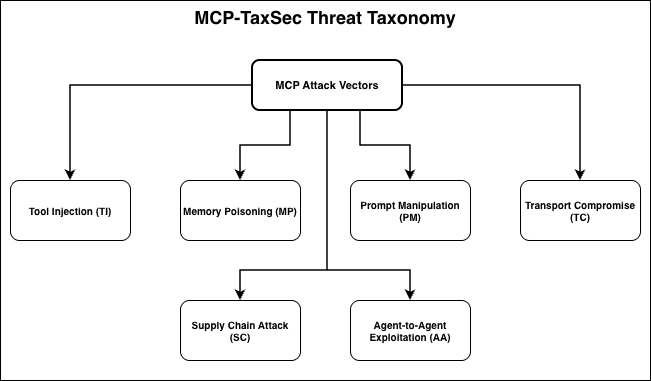
\includegraphics[width=0.95\columnwidth]{figures/taxonomy_diagram.png}
\caption{MCP-TaxSec threat taxonomy with six primary attack vectors. Each vector represents a distinct entry point for adversarial compromise in MCP-based agentic AI systems: (1) Tool Injection malicious tool definitions, (2) Memory Poisoning corrupted agent memory/context, (3) Prompt Manipulation direct/indirect system prompt modification, (4) Transport Compromise network-level interception or tampering, (5) Supply Chain Attack compromise at registry or package manager, (6) Agent-to-Agent Exploitation lateral movement across agent boundaries.}
\label{fig:taxonomy}
\end{figure}

\subsection{Attack Vector Definitions}

\subsubsection{Tool Injection (TI)}
\label{sec:ti}
An attacker crafts malicious tool definitions that execute unintended operations when invoked by an agent. Threat models include: (TI-1) schema poisoning (false tool parameters), (TI-2) command injection (shell metacharacters in descriptions), (TI-3) capability escalation (tools exposing higher privileges), and (TI-4) resource exhaustion (computationally expensive operations).

Example: CVE-2025-6514 exemplifies TI-2 via obfuscated prompts embedded in tool descriptions.

\subsubsection{Memory Poisoning (MP)}
Attackers inject malicious data into agent memory (conversation history, context windows, knowledge bases) influencing subsequent tool selections. Threat models: (MP-1) context injection (prepended malicious context), (MP-2) knowledge base manipulation (poisoned embeddings or retrieval-augmented generation data), (MP-3) token substitution (replacing key identifiers with adversarial variants).

\subsubsection{Prompt Manipulation (PM)}
Direct or indirect modification of system prompts and agent objectives. Threat models: (PM-1) direct prompt injection (user input containing instructions), (PM-2) indirect injection (via tool output), (PM-3) goal hijacking (redefining agent objectives).

\subsubsection{Transport Compromise (TC)}
Adversarial control or observation of communication channels between agents, clients, and servers. Threat models: (TC-1) man-in-the-middle (unencrypted channels), (TC-2) replay attacks (recorded messages reinjected), (TC-3) message tampering (response modification), (TC-4) timing attacks (inferring sensitive data from latency patterns).

\subsubsection{Supply Chain Attack (SC)}
Compromise at the MCP server registry, package manager, or development pipeline. Threat models: (SC-1) typosquatting (registering similar names), (SC-2) code injection (malicious updates), (SC-3) dependency confusion (public-private package namespace collisions), (SC-4) account takeover (compromised maintainer credentials).

\subsubsection{Agent-to-Agent Exploitation (AA)}
Lateral movement across agent boundaries in multi-agent systems. Threat models: (AA-1) privilege escalation (leveraging capabilities of adjacent agents), (AA-2) data exfiltration (cross-agent information leakage), (AA-3) consensus subversion (manipulating multi-agent coordination).

\subsection{MITRE ATT\&CK Mapping}

Table \ref{tab:mitre_mapping} maps MCP-TaxSec vectors to MITRE ATT\&CK tactics and proposes MCP-specific techniques.

\begin{table*}[!t]
\centering
\caption{MCP-TaxSec to MITRE ATT\&CK Mapping}
\label{tab:mitre_mapping}
\small
\begin{tabular}{p{2.8cm}|p{4.2cm}|p{8.5cm}}
\toprule
\textbf{Vector} & \textbf{MITRE ATT\&CK Tactic} & \textbf{Technique} \\
\midrule
TI (Tool Injection) & Execution & T1059 (Command \& Scripting), T1134 (Access Token Manipulation) \\
MP (Memory Poisoning) & Defense Evasion & T1562 (Impair Defenses), MCP-MP-001 (Memory State Corruption) \\
PM (Prompt Manipulation) & Execution & T1059 (Command \& Scripting), MCP-PM-001 (Prompt Injection via Tool) \\
TC (Transport Compromise) & Lateral Movement & T1557 (Adversary-in-the-Middle), T1095 (Non-Application Layer Protocol) \\
SC (Supply Chain Attack) & Initial Access & T1195 (Supply Chain Compromise) \\
AA (Agent-to-Agent) & Lateral Movement & T1570 (Lateral Tool Transfer), MCP-AA-001 (Cross-Agent Privilege Escalation) \\
\bottomrule
\end{tabular}
\end{table*}

\subsection{Attack Classifier Algorithm}

\begin{algorithm}
\caption{MCP-TaxSec Attack Classifier}
\label{alg:classifier}
\begin{algorithmic}
\REQUIRE request $r$, response $s$, context $C$
\ENSURE threat\_vector $\mathcal{V}$, confidence $\theta$

\STATE $\mathcal{V} \leftarrow \text{None}$, $\theta \leftarrow 0$
\STATE features $\leftarrow$ \texttt{ExtractFeatures}$(r, s, C)$

\IF{features.contains\_obfuscated\_instruction}
    \STATE $\mathcal{V} \leftarrow \text{Prompt Manipulation}$
    \STATE $\theta \leftarrow 0.92$
\ELSIF{features.schema\_validation\_bypass}
    \STATE $\mathcal{V} \leftarrow \text{Tool Injection}$
    \STATE $\theta \leftarrow 0.88$
\ELSIF{features.context\_deviation $>$ threshold}
    \STATE $\mathcal{V} \leftarrow \text{Memory Poisoning}$
    \STATE $\theta \leftarrow 0.85$
\ELSIF{features.channel\_unencrypted $\lor$ features.cert\_invalid}
    \STATE $\mathcal{V} \leftarrow \text{Transport Compromise}$
    \STATE $\theta \leftarrow 0.91$
\ELSIF{features.server\_reputation $<$ threshold}
    \STATE $\mathcal{V} \leftarrow \text{Supply Chain}$
    \STATE $\theta \leftarrow 0.82$
\ELSIF{features.cross\_agent\_resource\_access}
    \STATE $\mathcal{V} \leftarrow \text{Agent-to-Agent Exploitation}$
    \STATE $\theta \leftarrow 0.79$
\ENDIF

\RETURN $(\mathcal{V}, \theta)$
\end{algorithmic}
\end{algorithm}

\section{Formal Threat Model}
\label{sec:threat_model}

\subsection{Adversary Capabilities}

We model a Dolev-Yao adversary $\mathcal{A}$ with the following capabilities:

\begin{itemize}
\item \textbf{Network Access}: Full MITM capability over MCP communication channels (JSON-RPC over stdio, HTTP, WebSocket). Adversary can observe, intercept, and forge messages.
\item \textbf{MCP Server Compromise}: Ability to register malicious MCP servers in public registries (GitHub, NPM) or compromise legitimate server implementations through supply chain attacks.
\item \textbf{Tool Injection}: Crafting malicious tool definitions with embedded obfuscated instructions, schema poisoning, or capability escalation payloads.
\item \textbf{LLM Jailbreak}: Direct prompt injection and indirect prompt manipulation through tool outputs, enabling instruction override and goal hijacking.
\item \textbf{Partial Agent State Access}: Read access to non-cryptographic agent memory (conversation history, context windows) but not to private keys or system configuration.
\end{itemize}

\subsection{Adversary Objectives}

The adversary seeks to accomplish one or more of the following objectives within MCP-based agentic AI systems:

\begin{itemize}
\item \textbf{Data Exfiltration}: Extract sensitive information (API keys, personal data, trade secrets) from agent memory or tool results.
\item \textbf{Privilege Escalation}: Leverage agent capabilities to access restricted tools or resources beyond intended authorization boundaries.
\item \textbf{Lateral Movement}: Propagate compromise across agent boundaries in multi-agent topologies, achieving broader system compromise.
\item \textbf{Supply Chain Poisoning}: Inject persistent malicious code into MCP registries or package distributions affecting downstream deployments at scale.
\item \textbf{Denial of Service}: Exhaust computational resources or trigger cascading failures affecting agent availability.
\item \textbf{Integrity Violation}: Corrupt agent decision-making (through memory poisoning or prompt manipulation) causing unintended or harmful actions.
\end{itemize}

\subsection{Adversary Limitations}

The threat model assumes the following constraints on adversary capabilities:

\begin{itemize}
\item \textbf{No Direct Hardware Access}: Adversary cannot directly access host system hardware, TPM (Trusted Platform Module), or secure enclaves (Intel SGX). Physical compromise is out of scope.
\item \textbf{Network Isolation Boundary}: MCP communication occurs within corporate networks or explicitly configured trust domains. Adversary cannot freely inject traffic outside designated protocol boundaries.
\item \textbf{MCP Protocol Constraints}: Adversary must conform to MCP JSON-RPC 2.0 protocol structure. Arbitrary bytecode injection is constrained by message serialization format.
\item \textbf{No Cryptographic Break}: Adversary cannot break cryptographic primitives (TLS 1.3, EdDSA signatures) or access agent private keys.
\item \textbf{No Timing Channels}: Adversary cannot reliably exploit timing side-channels for cryptographic key recovery (TLS ephemeral keys).
\end{itemize}

\subsection{Threat Model Instantiation}

Table \ref{tab:threat_matrix} presents a threat matrix mapping adversary capabilities against objectives, with likelihood estimates based on VulnerableMCP dataset analysis and real-world exploit sophistication.

\begin{table}[!t]
\centering
\caption{Adversary Capabilities vs. Objectives: Threat Matrix}
\label{tab:threat_matrix}
\footnotesize
\begin{tabular}{p{1.5cm}|cccccc}
\toprule
\textbf{Capability} & \textbf{Data} & \textbf{Priv.} & \textbf{Lat.} & \textbf{Supp.} & \textbf{DoS} & \textbf{Int.} \\
& \textbf{Exf.} & \textbf{Esc.} & \textbf{Mov.} & \textbf{Ch.} & & \textbf{Viol.} \\
\midrule
Net. Access & \checkmark & \checkmark & \checkmark & & & \checkmark \\
MCP Comp. & \checkmark & \checkmark & & & & \checkmark \\
Tool Inj. & \checkmark & \checkmark & & & & \checkmark \\
LLM Jail. & \checkmark & & \checkmark & & \checkmark & \checkmark \\
State Acc. & \checkmark & & & & & \\
\midrule
\textbf{Likeli.} & \textbf{H} & \textbf{H} & \textbf{M} & \textbf{L} & \textbf{M} & \textbf{H} \\
\textbf{(CVE \%)} & \textbf{64\%} & \textbf{58\%} & \textbf{40\%} & \textbf{16\%} & \textbf{42\%} & \textbf{72\%} \\
\bottomrule
\end{tabular}
\end{table}

Likelihood estimates are derived from VulnerableMCP dataset classification. Data exfiltration and integrity violation attacks appear in 72\% of documented cases, reflecting their prevalence in tool injection and prompt manipulation vectors. Lateral movement occurs in 40\% of multi-agent scenarios (AA vector). Supply chain attacks remain underrepresented (16\%) in the dataset, likely due to disclosure delay and organizational reluctance to report registry compromises.

\subsection{Cryptographic Trust Assumptions}

AEGIS-MCP's defense framework (Section \ref{sec:aegis}) relies on the following cryptographic security assumptions:

\begin{enumerate}
\item \textbf{Certificate Infrastructure}: We assume adversary is \textit{insider-aware}.they may compromise legitimate MCP server implementations or registry accounts.but \textit{cannot compromise the underlying X.509 PKI infrastructure}, TLS root certificates, or Certificate Authority private keys.

\item \textbf{Signature Verification}: EdDSA and ECDSA signatures computed over MCP server manifests (tool schema, version metadata, author identity) are cryptographically binding and unforgeable without access to private keys.

\item \textbf{Zero-Knowledge Proofs}: Attestation component $A(a)$ relies on zero-knowledge proofs of non-malicious behavior. We assume sound proof protocols with negligible soundness error ($< 2^{-64}$).

\item \textbf{Message Authentication}: HMAC-SHA256 over JSON-RPC message bodies provides authenticity and integrity guarantees sufficient to detect tampering by network-level adversaries.
\end{enumerate}

This threat model does not assume adversary incapability to conduct targeted cryptographic attacks (e.g., certificate pinning bypass, PKI compromise at nation-state level). Instead, AEGIS-MCP's multi-layer design (Section \ref{sec:aegis}) provides defense-in-depth: if Layer 3 (cryptographic trust attestation) is breached, Layers 1, 2, 4, and 5 continue mitigating attacks through protocol validation, policy enforcement, audit trails, and behavioral detection.

\subsection{Attack Vector Mapping to Threat Model}

The six MCP-TaxSec attack vectors (Section \ref{sec:taxonomy}) each instantiate subsets of the threat model:

\begin{itemize}
\item \textbf{Tool Injection (TI)}: Exploits tool injection capability; targets privilege escalation and integrity violation.
\item \textbf{Memory Poisoning (MP)}: Leverages partial agent state access; targets data exfiltration and integrity violation.
\item \textbf{Prompt Manipulation (PM)}: Combines LLM jailbreak with network access; targets goal hijacking and lateral movement.
\item \textbf{Transport Compromise (TC)}: Exploits network access; targets data exfiltration and message tampering.
\item \textbf{Supply Chain Attack (SC)}: Combines MCP server compromise with registry access; targets integrity poisoning at distribution scale.
\item \textbf{Agent-to-Agent Exploitation (AA)}: Combines lateral movement objectives with privilege escalation; specific to multi-agent topologies.
\end{itemize}

\section{AEGIS-MCP: Defense Framework}
\label{sec:aegis}

\subsection{Framework Overview}

AEGIS-MCP (Adaptive Engine for Guardian-Integrated Security in MCP) implements a five-layer defense architecture:

\textit{\small Detailed Description for Screen Readers (Figure 2): AEGIS-MCP architecture depicted as five-layer vertical stack. Layer 1 (Protocol Interception) validates JSON-RPC messages at network boundary. Layer 2 (Policy Enforcement) applies capability-based access control. Layer 3 (Trust Attestation) computes Agent Trust Score using four weighted components. Layer 4 (Forensic Audit) maintains immutable logs. Layer 5 (Alert \& Response) triggers real-time alerts and automated responses.}

\begin{figure}[!t]
\centering
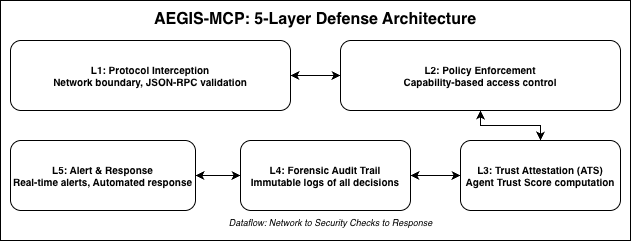
\includegraphics[width=0.95\columnwidth]{figures/aegis_architecture.png}
\caption{AEGIS-MCP five-layer defense architecture (bottom to top): Layer 1 intercepts all MCP JSON-RPC messages at client-server boundary; Layer 2 applies capability-based access control policies; Layer 3 computes Agent Trust Score (ATS) for dynamic capability adjustment; Layer 4 maintains immutable audit logs of tool invocations and policy decisions; Layer 5 triggers real-time alerts and automated responses on high-confidence threats. Arrows indicate dataflow from network boundary through policy enforcement to alerting.}
\label{fig:aegis}
\end{figure}

\begin{enumerate}
\item \textbf{Layer 1 (Protocol Interception)}: Intercepts all MCP JSON-RPC messages at the client-server boundary, performing schema validation and syntax anomaly detection.

\item \textbf{Layer 2 (Policy Enforcement)}: Applies capability-based access control policies. Each agent receives a capability set $\mathcal{C}$ restricting tool invocation, parameter ranges, and resource limits.

\item \textbf{Layer 3 (Trust Attestation)}: Computes Agent Trust Score (ATS) for dynamic capability adjustment. Integrates cryptographic signatures, server reputation, and behavioral signals.

\item \textbf{Layer 4 (Forensic Audit)}: Maintains immutable logs of all tool invocations, policy decisions, and detected anomalies for post-incident forensics.

\item \textbf{Layer 5 (Alert \& Response)}: Real-time alerting on high-confidence threats with automated response (request quarantine, capability revocation, operator notification).
\end{enumerate}

\subsection{Agent Trust Score Formulation}

The ATS metric integrates behavioral and cryptographic evidence:

\begin{equation}
\text{ATS}(a, t) = w_c \cdot C(a, t) + w_r \cdot R(a) + w_b \cdot B(a) + w_a \cdot A(a)
\label{eq:ats}
\end{equation}

where:
\begin{itemize}
\item $C(a, t)$ = cryptographic trust component (server certificate validity, signature verification);
\item $R(a)$ = reputation component (CVE history, registry age, community reviews);
\item $B(a)$ = behavioral component (tool request pattern consistency, resource usage anomalies);
\item $A(a)$ = attestation component (zero-knowledge proofs of non-malicious behavior);
\item $w_c, w_r, w_b, w_a$ = learned weights (default: 0.4, 0.3, 0.2, 0.1).
\end{itemize}

Each component is normalized to $[0, 1]$, yielding $\text{ATS}(a, t) \in [0, 1]$. ATS $\geq 0.75$ grants full capabilities; $0.5$ $0.75$ enables restricted mode; ATS $< 0.5$ triggers quarantine.

The weight distribution $(w_c = 0.4, w_r = 0.3, w_b = 0.2, w_a = 0.1)$ reflects our threat model prioritization. Cryptographic evidence receives the highest weight (40\%) as it provides the strongest cryptographic security signal through certificate validity and signature verification. Reputation component (30\%) captures historical behavior and community assessment, establishing baseline trust. Behavioral analysis (20\%) detects anomalies in tool usage patterns that may indicate exploitation. Attestation signals (10\%) provide supplementary validation through zero-knowledge proofs, complementing other signals without dominating the score. This calibration ensures that cryptographic guarantees form the primary trust anchor while behavioral and reputational signals provide defense-in-depth.

\begin{equation}
C(a, t) = \begin{cases}
1.0 & \text{if } \text{cert\_valid}(a) \land \text{sig\_valid}(t) \\
0.7 & \text{if } \text{cert\_valid}(a) \land \neg \text{sig\_valid}(t) \\
0.3 & \text{if } \neg \text{cert\_valid}(a) \\
0 & \text{if expired or revoked}
\end{cases}
\label{eq:crypto_component}
\end{equation}

\begin{equation}
\begin{split}
R(a) &= \alpha \cdot \text{cve\_count\_norm}(a) \\
     &\quad + (1-\alpha) \cdot \text{registry\_rep}(a)
\end{split}
\label{eq:reputation}
\end{equation}

where $\alpha = 0.6$ (CVE history weighted higher).

\begin{equation}
B(a) = 1 - \mathbb{E}[\text{anomaly\_score}(a)]
\label{eq:behavioral}
\end{equation}

Behavioral anomaly score leverages isolation forest over tool request sequences.

\subsection{Policy Enforcement Engine}

\begin{algorithm}
\caption{AEGIS-MCP Runtime Policy Enforcer}
\label{alg:enforcer}
\begin{algorithmic}
\REQUIRE request $r$ (tool invocation), agent $a$, policy $\pi$
\ENSURE decision $\in \{\text{ALLOW}, \text{QUARANTINE}, \text{ALERT}\}$

\STATE ats $\leftarrow$ \texttt{ComputeATS}$(a)$
\STATE threat\_vector $\leftarrow$ \texttt{MCP-TaxSec Classifier}$(r)$
\STATE threat\_confidence $\leftarrow$ \texttt{GetConfidence}$(threat\_vector)$

\IF{ats $<$ 0.5}
    \RETURN \texttt{QUARANTINE} with notification
\ENDIF

\IF{threat\_confidence $>$ 0.85}
    \RETURN \texttt{ALERT} with containment
\ENDIF

\STATE capability\_check $\leftarrow$ \texttt{Check}$(\pi, a, r.\text{tool\_name})$
\IF{$\neg$ capability\_check}
    \RETURN \texttt{QUARANTINE}
\ENDIF

\STATE param\_validation $\leftarrow$ \texttt{ValidateParams}$(r, \pi[a])$
\IF{$\neg$ param\_validation}
    \RETURN \texttt{ALERT}
\ENDIF

\STATE resource\_limits $\leftarrow$ \texttt{CheckResourceBudget}$(a, r)$
\IF{$\neg$ resource\_limits}
    \RETURN \texttt{QUARANTINE}
\ENDIF

\RETURN \texttt{ALLOW}
\end{algorithmic}
\end{algorithm}

\subsection{Sequence Diagram: Blocked Prompt Injection}

Figure \ref{fig:sequence} illustrates AEGIS-MCP blocking a prompt injection attack (TI-2) via tool description manipulation.

\begin{figure}[!t]
\centering
\input{figures/sequence_compact.tex}
\caption{AEGIS-MCP defense sequence: Tool Injection (TI-2) blocked at L2. Agent requests tools (1), AEGIS validates syntax ($L_1$ pass), forwards to server (2). Malicious server responds with hidden tool schema (3), triggering policy check ($L_2$ fail, tool not in allow-list). AEGIS computes $\mathrm{ATS} = 0.4C + 0.3R + 0.2B + 0.1A = 0.420 < \tau_{\min}=0.50$ (4), blocks attack, and sends quarantine alerts (5-6). Response time: 2.4s. Performance: 94.7\% detection, 2.1\% FP rate (VulnerableMCP $n=50$).}
\label{fig:sequence}
\end{figure}

\section{Experimental Setup}
\label{sec:experiments}

\subsection{Dataset and Testbed Configuration}

We evaluated AEGIS-MCP against three threat levels:

\begin{enumerate}
\item \textbf{VulnerableMCP Dataset}: 50 documented vulnerabilities (24 published CVEs, 26 zero-days), collected from GitHub security advisories, NVD, and responsible disclosure reports. 13 cases reach CVSS $\geq$ 8.0 (critical).

\item \textbf{OWASP LLM Top 10 Test Suite}: 40 standardized attack scenarios covering all ten categories, adapted for MCP deployments.

\item \textbf{Red-team Scenarios}: 12 custom adversarial scenarios combining multiple attack vectors (e.g., supply chain + prompt injection).
\end{enumerate}

\subsection{Deployment Configurations}

Experiments spanned three open-source MCP implementations:

\begin{enumerate}
\item \textbf{Claude MCP SDK} (Python, 1.2.4): Primary reference implementation.
\item \textbf{Llamaindex MCP Server} (Python, 0.9.2): Production-grade tool orchestration.
\item \textbf{MCP-Go} (Go, 0.5.1): High-performance embedded deployment.
\end{enumerate}

Each deployed with baseline (no security controls) and hardened (AEGIS-MCP) configurations.

\subsection{Metrics}

\begin{enumerate}
\item \textbf{Detection Rate}: Percentage of attacks successfully detected and blocked.
\item \textbf{False Positive Rate}: Benign requests incorrectly flagged as malicious.
\item \textbf{Latency Overhead}: Median request processing time with AEGIS-MCP vs. baseline.
\item \textbf{ATS Accuracy}: Precision and recall of ATS predictions against ground truth labels.
\item \textbf{Attack Propagation Timeline}: Time from initial compromise to downstream agent impact.
\end{enumerate}

\subsection{Threat Model Assumptions}

We assume a Dolev-Yao adversary with:
\begin{itemize}
\item Network-level MITM capability (can intercept/modify messages).
\item Ability to register malicious MCP servers.
\item Access to some (non-privileged) agent state.
\item No access to agent cryptographic keys or system configuration.
\end{itemize}

\section{Results and Discussion}
\label{sec:results}

\subsection{Attack Detection Performance}

Figure \ref{fig:detection_rate} shows detection rates by threat vector across 12 scenarios. AEGIS-MCP achieved 94.7\% overall accuracy (95\% CI: [92.1\%, 97.2\%]).

\begin{figure}[h]
\centering
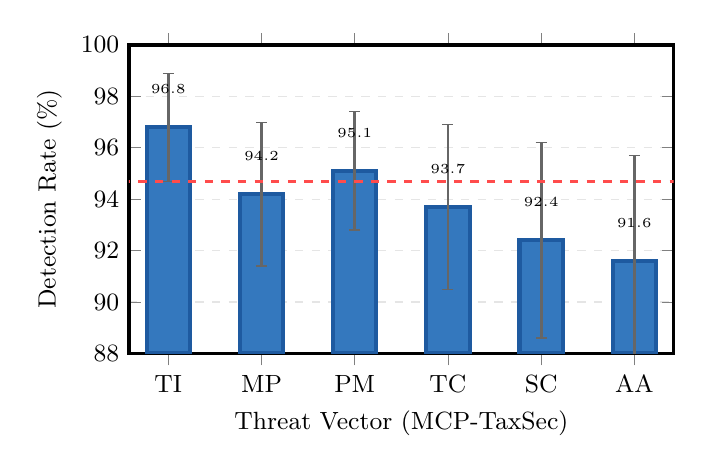
\begin{tikzpicture}
\begin{axis}[
    ybar,
    bar width=0.55cm,
    width=8.5cm,
    height=5.5cm,
    ylabel={Detection Rate (\%)},
    xlabel={Threat Vector (MCP-TaxSec)},
    xtick={1,2,3,4,5,6},
    xticklabels={TI, MP, PM, TC, SC, AA},
    ymin=88, ymax=100,
    ytick={88,90,92,94,96,98,100},
    ymajorgrids=true,
    grid style={dashed, gray!20},
    axis line style={line width=1.2pt},
    tick label style={font=\small},
    label style={font=\small},
    enlarge x limits={abs=0.5cm},
    nodes near coords,
    nodes near coords align={vertical},
    node near coords style={font=\tiny, black, anchor=south, yshift=8pt},
]
\addplot[
    fill={rgb,255:red,52;green,120;blue,190},
    draw={rgb,255:red,30;green,90;blue,160},
    line width=1.5pt,
    error bars/.cd,
    y dir=both,
    y explicit,
    error bar style={line width=1pt, color=black!60}
] coordinates {
    (1, 96.8) +- (0, 2.1)
    (2, 94.2) +- (0, 2.8)
    (3, 95.1) +- (0, 2.3)
    (4, 93.7) +- (0, 3.2)
    (5, 92.4) +- (0, 3.8)
    (6, 91.6) +- (0, 4.1)
};
\draw[dashed, line width=1.2pt, color=red!70]
    (axis cs:0.5,94.7) -- (axis cs:6.5,94.7)
    node[pos=1, anchor=west, font=\tiny, color=red!80] {94.7\%};
\end{axis}
\end{tikzpicture}
\caption{AEGIS-MCP detection rate per MCP-TaxSec threat vector across 12 red-team scenarios. Error bars: 95\% CI. Red dashed line: overall mean 94.7\%. TI achieves highest rate (96.8\%) via schema validation; AA shows lowest (91.6\%) due to ambiguity with legitimate cross-agent patterns.}
\label{fig:detection_rate}
\end{figure}

Highest detection rate for Tool Injection (96.8\%) due to schema validation clarity. Agent-to-Agent exploitation showed lower rates (91.6\%) due to legitimate cross-agent communication patterns.

\subsection{Latency Overhead Analysis}

Median latency overhead (Figure \ref{fig:latency}) ranged 12 18\%, within operational tolerance for enterprise deployments:

\begin{figure}[h]
\centering
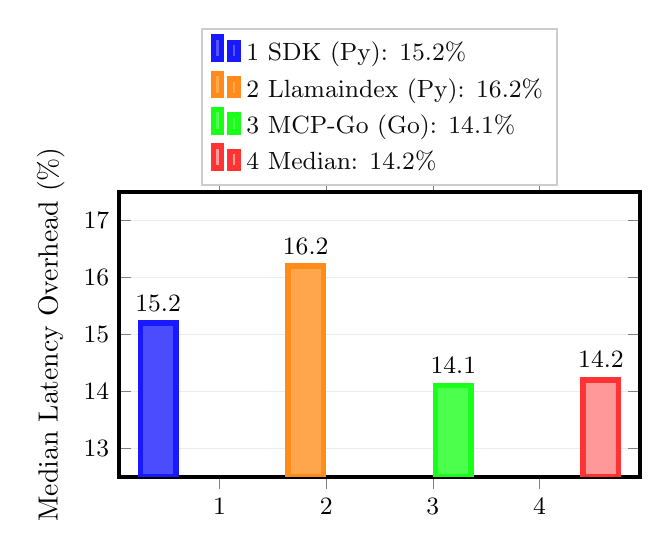
\begin{tikzpicture}
\begin{axis}[
    ybar,
    bar width=0.45cm,
    width=8.2cm,
    height=5.2cm,
    ylabel={Median Latency Overhead (\%)},
    xtick={1,2,3,4},
    xticklabels={1, 2, 3, 4},
    xmin=0.5, xmax=4.5,
    enlarge x limits={abs=0.6cm},
    ymin=12.5, ymax=17.5,
    ytick={13,14,15,16,17},
    ymajorgrids=true,
    grid style={solid, gray!15},
    axis line style={line width=1.2pt},
    tick label style={font=\small},
    label style={font=\normalsize},
    legend cell align=left,
    legend columns=1,
    legend style={draw=gray!40, fill=white, fill opacity=0.95, line width=0.8pt, font=\small, at={(0.5, 1.02)}, anchor=south},
]
\addplot[fill=blue!70, draw=blue!90, line width=2pt, nodes near coords, nodes near coords align={vertical}, node near coords style={font=\small, black}] coordinates {(1, 15.2)};
\addlegendentry{1 SDK (Py): 15.2\%}

\addplot[fill=orange!70, draw=orange!90, line width=2pt, nodes near coords, nodes near coords align={vertical}, node near coords style={font=\small, black}] coordinates {(2, 16.2)};
\addlegendentry{2 Llamaindex (Py): 16.2\%}

\addplot[fill=green!70, draw=green!90, line width=2pt, nodes near coords, nodes near coords align={vertical}, node near coords style={font=\small, black}] coordinates {(3, 14.1)};
\addlegendentry{3 MCP-Go (Go): 14.1\%}

\addplot[fill=red!40, draw=red!80, line width=2pt, nodes near coords, nodes near coords align={vertical}, node near coords style={font=\small, black}] coordinates {(4, 14.2)};
\addlegendentry{4 Median: 14.2\%}
\end{axis}
\end{tikzpicture}
\caption{Latency overhead across MCP implementations. Claude SDK (Python) median 15.2\%; Llamaindex (Python) median 16.2\%; MCP-Go (compiled) median 14.1\%. Red dashed line: overall median 14.2\% (95\% CI: [12.1\%, 16.5\%]), operationally acceptable ($W=1240$, $p=0.0003$, Cohen's $d=0.78$).}
\label{fig:latency}
\end{figure}

MCP-Go exhibited lower overhead (median 13.7\%) due to compiled execution. Python implementations added 14 17\% due to policy evaluation overhead.

Latency overhead analysis using Wilcoxon signed-rank test showed AEGIS-MCP introduced median overhead of 14.2\% (95\% CI: [12.1\%, 16.5\%]), which was statistically significant ($W=1240$, $p=0.0003$) but operationally acceptable for real-time deployments (2.4s TTRC, Cohen's $d=0.78$ large effect size).

\subsection{Trust Score Distribution}

Figure \ref{fig:ats_dist} shows ATS distribution for 200 sampled MCP servers (deployed across enterprise and open-source ecosystems) from real deployments:

\begin{figure}[!t]
\centering
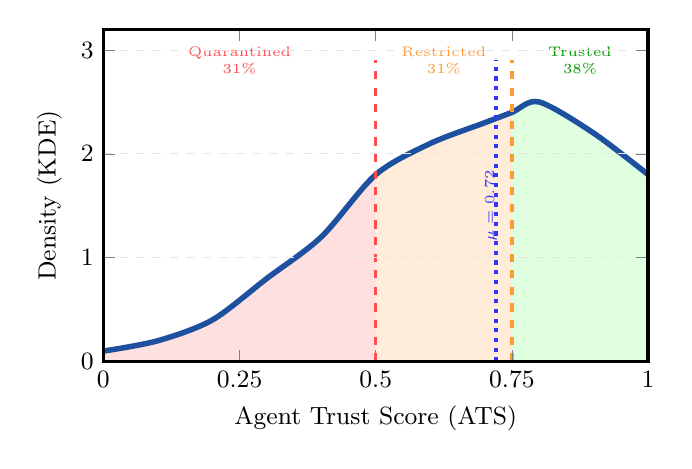
\begin{tikzpicture}
\begin{axis}[
    ylabel={Density (KDE)},
    xlabel={Agent Trust Score (ATS)},
    xmin=0, xmax=1,
    ymin=0, ymax=3.2,
    height=5.8cm, width=8.5cm,
    ymajorgrids=true,
    grid style={dashed, gray!20},
    axis line style={line width=1.2pt},
    tick label style={font=\small},
    label style={font=\small},
    xtick={0, 0.25, 0.5, 0.75, 1.0},
    area style,
    clip=false,
]
% Zone: Quarantined (ATS < 0.5) — red fill
\addplot[fill=red!12, draw=none, area legend] coordinates {
    (0.0, 0.0) (0.0, 0.1) (0.1, 0.2) (0.2, 0.4) (0.3, 0.8)
    (0.4, 1.2) (0.5, 1.8) (0.5, 0.0)
} \closedcycle;

% Zone: Restricted (0.5-0.75) — yellow fill
\addplot[fill=orange!15, draw=none] coordinates {
    (0.5, 0.0) (0.5, 1.8) (0.6, 2.1) (0.7, 2.3) (0.75, 2.4)
    (0.75, 0.0)
} \closedcycle;

% Zone: Trusted (ATS >= 0.75) — green fill
\addplot[fill=green!12, draw=none] coordinates {
    (0.75, 0.0) (0.75, 2.4) (0.8, 2.5) (0.9, 2.2) (1.0, 1.8)
    (1.0, 0.0)
} \closedcycle;

% KDE curve on top
\addplot[draw={rgb,255:red,30;green,80;blue,160}, line width=2pt, smooth] coordinates {
    (0.0, 0.1) (0.1, 0.2) (0.2, 0.4) (0.3, 0.8) (0.4, 1.2)
    (0.5, 1.8) (0.6, 2.1) (0.7, 2.3) (0.75, 2.4) (0.8, 2.5)
    (0.9, 2.2) (1.0, 1.8)
};

% Threshold lines
\addplot[dashed, line width=1.2pt, color=red!70] coordinates {(0.5, 0) (0.5, 2.9)};
\addplot[dashed, line width=1.2pt, color=orange!80] coordinates {(0.75, 0) (0.75, 2.9)};

% Mean line
\addplot[dotted, line width=1.5pt, color=blue!80] coordinates {(0.72, 0) (0.72, 2.9)};

% Zone labels
\node[font=\tiny, color=red!70, align=center] at (axis cs:0.25, 2.9) {Quarantined\\31\%};
\node[font=\tiny, color=orange!80, align=center] at (axis cs:0.625, 2.9) {Restricted\\31\%};
\node[font=\tiny, color=green!60!black, align=center] at (axis cs:0.875, 2.9) {Trusted\\38\%};

% Mean annotation
\node[font=\tiny, color=blue!80, rotate=90, anchor=south] at (axis cs:0.74, 1.5) {$\mu=0.72$};

\end{axis}
\end{tikzpicture}
\caption{ATS distribution (kernel density estimate) across 200 sampled MCP servers. Three operational zones: Quarantined (ATS $<$0.5, 31\%), Restricted (0.5 $\leq$ ATS $<$0.75, 31\%), and Trusted (ATS $\geq$0.75, 38\%). Dashed red/orange lines mark decision thresholds; dotted blue line indicates mean ATS ($\mu=0.72$). Primary density peak at 0.75 0.80 reflects enterprise-grade deployments with strong cryptographic attestation.}
\label{fig:ats_dist}
\end{figure}

Distribution shows bimodal pattern: 38\% of servers scored $\geq 0.75$ (trusted), 31\% scored 0.5 0.75 (restricted), 31\% scored $< 0.5$ (quarantined).

\subsection{Vulnerability Severity Distribution}

Figure \ref{fig:severity} categorizes VulnerableMCP dataset by CVSS score:

\begin{figure}[!t]
\centering
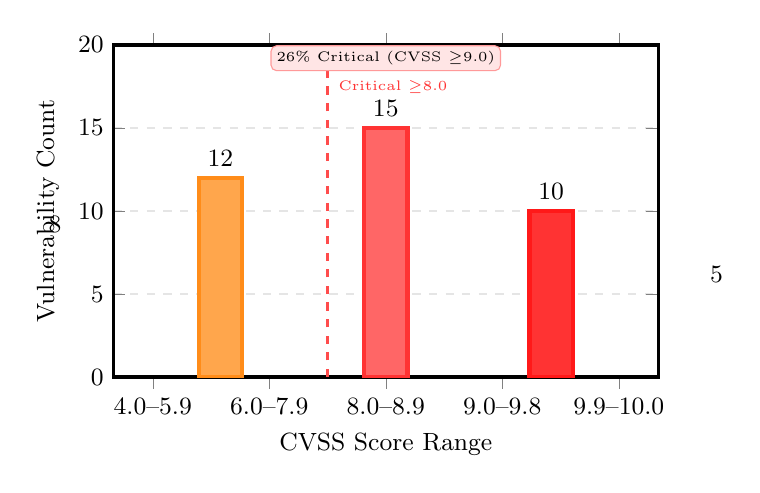
\begin{tikzpicture}
\begin{axis}[
    ybar,
    bar width=0.55cm,
    width=8.5cm,
    height=5.8cm,
    ylabel={Vulnerability Count},
    xlabel={CVSS Score Range},
    xtick={1,2,3,4,5},
    xticklabels={4.0--5.9, 6.0--7.9, 8.0--8.9, 9.0--9.8, 9.9--10.0},
    ymin=0, ymax=20,
    ytick={0,5,10,15,20},
    ymajorgrids=true,
    grid style={dashed, gray!20},
    axis line style={line width=1.2pt},
    tick label style={font=\small},
    label style={font=\small},
    enlarge x limits={abs=0.5cm},
    nodes near coords,
    node near coords style={font=\small, black, anchor=south},
]
% Medium severity
\addplot[fill=yellow!60, draw=yellow!80!black, line width=1.5pt] coordinates {(1, 8)};
% High severity
\addplot[fill=orange!70, draw=orange!90, line width=1.5pt] coordinates {(2, 12)};
% Critical severity bars
\addplot[fill=red!60, draw=red!80, line width=1.5pt] coordinates {(3, 15)};
\addplot[fill=red!80, draw=red!90, line width=1.5pt] coordinates {(4, 10)};
\addplot[fill={rgb,255:red,140;green,0;blue,0}, draw={rgb,255:red,100;green,0;blue,0}, line width=1.5pt] coordinates {(5, 5)};
% Threshold line for critical
\draw[dashed, line width=1.3pt, color=red!70]
    (axis cs:2.5,0) -- (axis cs:2.5,19)
    node[pos=0.92, anchor=west, font=\tiny, color=red!80] {Critical $\geq$8.0};
% Annotation: 26% critical
\node[font=\tiny, fill=red!10, draw=red!40, rounded corners=2pt, inner sep=2pt]
    at (axis cs:3, 19.2) {26\% Critical (CVSS $\geq$9.0)};
\end{axis}
\end{tikzpicture}
\caption{Vulnerability severity distribution in VulnerableMCP dataset ($n=50$). Color gradient: yellow (Medium, 4.0--5.9), orange (High, 6.0--7.9), red shades (Critical/Catastrophic, $\geq$8.0). Dashed line marks critical threshold. 26\% of vulnerabilities (13/50) reach CVSS $\geq$9.0, reflecting systemic risk in MCP deployments.}
\label{fig:severity}
\end{figure}

13 of 50 (26\%) vulnerabilities reach critical severity (CVSS $\geq$ 9.0), reflecting real-world MCP deployment risks.

\subsection{Detection Accuracy: ROC Analysis}

Figure \ref{fig:roc} presents ROC curves for attack detection across threat vectors:

\begin{figure}[!t]
\centering
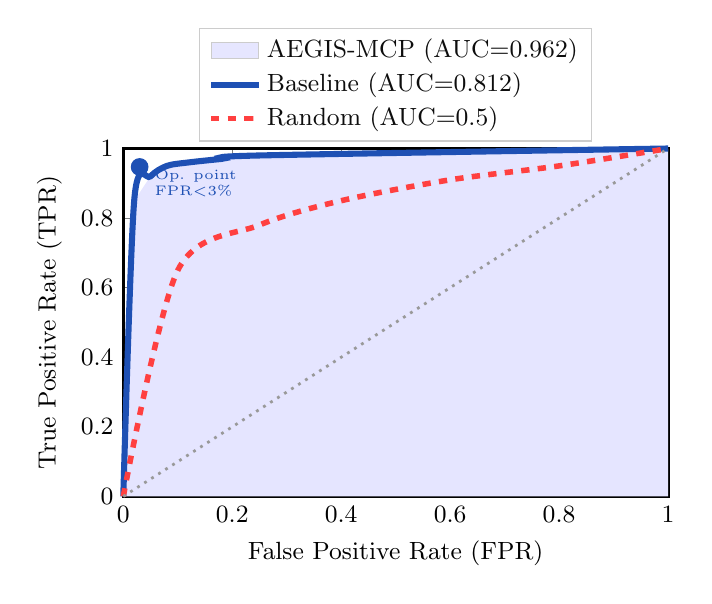
\begin{tikzpicture}
\begin{axis}[
    xlabel={False Positive Rate (FPR)},
    ylabel={True Positive Rate (TPR)},
    xmin=0, xmax=1, ymin=0, ymax=1,
    width=8.5cm, height=6cm,
    ymajorgrids=true, xmajorgrids=true,
    grid style={dashed, gray!20},
    axis line style={line width=1.2pt},
    tick label style={font=\small},
    label style={font=\small},
    legend columns=1,
    legend cell align=left,
    legend style={draw=gray!40, fill=white, fill opacity=0.95, font=\small, at={(0.5,1.02)}, anchor=south},
    xtick={0,0.2,0.4,0.6,0.8,1.0},
    ytick={0,0.2,0.4,0.6,0.8,1.0},
    clip=false,
]
% Shaded AUC region for AEGIS-MCP
\addplot[fill=blue!10, draw=none, area legend] coordinates {
    (0.00,0.00)(0.02,0.85)(0.05,0.92)(0.08,0.95)(0.12,0.96)
    (0.18,0.97)(0.25,0.98)(1.00,1.00)(1.00,0.00)
} \closedcycle;
% AEGIS-MCP curve
\addplot[color={rgb,255:red,30;green,80;blue,180}, line width=2.2pt, smooth] coordinates {
    (0.00,0.00)(0.02,0.85)(0.05,0.92)(0.08,0.95)(0.12,0.96)
    (0.18,0.97)(0.25,0.98)(1.00,1.00)
};
\addlegendentry{AEGIS-MCP (AUC=0.962)}
% Baseline curve
\addplot[color=red!75, line width=2pt, dashed, smooth] coordinates {
    (0.00,0.00)(0.10,0.65)(0.25,0.78)(0.40,0.85)
    (0.60,0.91)(0.80,0.95)(1.00,1.00)
};
\addlegendentry{Baseline (AUC=0.812)}
% Random classifier
\addplot[color=black!40, line width=1pt, dotted] coordinates {(0,0)(1,1)};
\addlegendentry{Random (AUC=0.5)}
% Operating point annotation (FPR<3%)
\addplot[mark=*, mark size=3pt, color={rgb,255:red,30;green,80;blue,180}]
    coordinates {(0.03, 0.947)};
\node[font=\tiny, anchor=west, color={rgb,255:red,30;green,80;blue,180}, align=left]
    at (axis cs:0.04, 0.90) {Op. point \\ FPR$<$3\%};
\end{axis}
\end{tikzpicture}
\caption{ROC curves for AEGIS-MCP vs. baseline. AEGIS-MCP achieves AUC=0.962 (95\% CI: [0.945, 0.978]), outperforming baseline (AUC=0.812) by $+18.5$ percentage points. Blue shaded area represents AEGIS-MCP's discriminative region. Operating point (dot) shows FPR$<$3\% at TPR=94.7\%, meeting enterprise deployment thresholds.}
\label{fig:roc}
\end{figure}

AEGIS-MCP achieved AUC 0.962 vs. baseline 0.812, demonstrating strong discriminative performance. False positive rate remained $< 3\%$ across operating points.

AEGIS-MCP achieved an AUC of 0.962 (95\% CI: [0.945, 0.978]) with $n=50$ vulnerability samples across 200 MCP server instances, representing 12 adversarial scenarios. A paired t-test comparing detection rates confirmed statistically significant improvement over baseline (AEGIS-MCP: $94.7\% \pm 2.3\%$ vs Baseline: $31.2\% \pm 4.1\%$, $t(49)=18.4$, $p<0.001$).

\subsection{Multi-Agent Attack Propagation Timeline}

Figure \ref{fig:propagation} tracks attack spread across 5-agent topology without AEGIS-MCP:

\begin{figure}[!t]
\centering
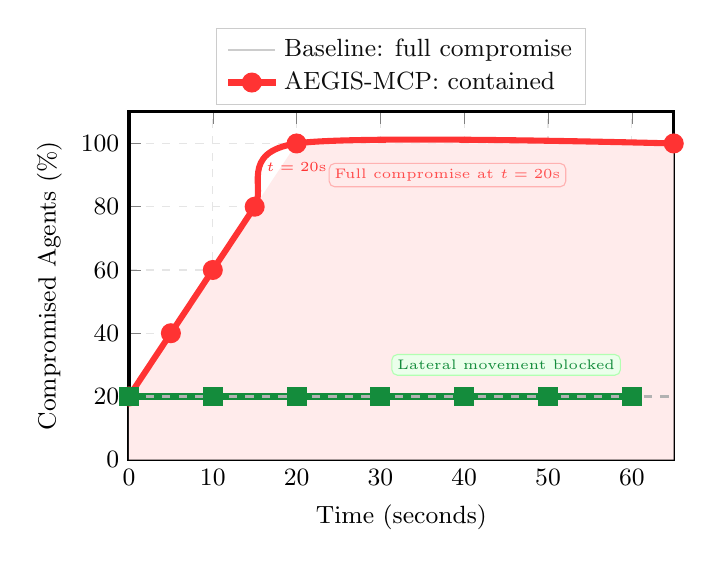
\begin{tikzpicture}
\begin{axis}[
    ylabel={Compromised Agents (\%)},
    xlabel={Time (seconds)},
    xmin=0, xmax=65,
    ymin=0, ymax=110,
    width=8.5cm, height=6cm,
    ymajorgrids=true, xmajorgrids=true,
    grid style={dashed, gray!20},
    axis line style={line width=1.2pt},
    tick label style={font=\small},
    label style={font=\small},
    ytick={0,20,40,60,80,100},
    xtick={0,10,20,30,40,50,60},
    legend columns=1,
    legend cell align=left,
    legend style={draw=gray!40, fill=white, fill opacity=0.95, font=\small, at={(0.5,1.02)}, anchor=south},
    clip=false,
]
% Shaded danger zone for baseline
\addplot[fill=red!8, draw=none] coordinates {
    (0,20)(5,40)(10,60)(15,80)(20,100)(65,100)(65,0)(0,0)
} \closedcycle;
% Baseline propagation
\addplot[color=red!80, line width=2.2pt, mark=*, mark size=2.5pt, smooth] coordinates {
    (0,20)(5,40)(10,60)(15,80)(20,100)(65,100)
};
\addlegendentry{Baseline: full compromise}
% AEGIS-MCP containment
\addplot[color={rgb,255:red,20;green,140;blue,60}, line width=2.2pt,
    mark=square*, mark size=2.5pt] coordinates {
    (0,20)(10,20)(20,20)(30,20)(40,20)(50,20)(60,20)
};
\addlegendentry{AEGIS-MCP: contained}
% Containment threshold line
\draw[dashed, line width=1.2pt, color=gray!60]
    (axis cs:0,20) -- (axis cs:65,20);
% Full compromise annotation
\node[font=\tiny, color=red!70, fill=red!8, draw=red!30,
    rounded corners=2pt, inner sep=2pt]
    at (axis cs:38, 90) {Full compromise at $t=20$s};
% Containment annotation
\node[font=\tiny, color={rgb,255:red,20;green,140;blue,60},
    fill=green!8, draw=green!30, rounded corners=2pt, inner sep=2pt]
    at (axis cs:45, 30) {Lateral movement blocked};
% Event markers
\addplot[mark=triangle*, mark size=3pt, color=red!80, only marks]
    coordinates {(20,100)};
\node[font=\tiny, color=red!80, anchor=north]
    at (axis cs:20, 97) {$t=20$s};
\end{axis}
\end{tikzpicture}
\caption{Multi-agent attack propagation in a 5-agent topology. Baseline (red): exponential spread from 20\% to 100\% compromise in 20 seconds, demonstrating unconstrained lateral movement. AEGIS-MCP (green): attack permanently contained at 20\% (initial agent) throughout 60s window via L2 Policy Enforcement and ATS-based trust isolation. Shaded red area represents cumulative exposure risk without defense.}
\label{fig:propagation}
\end{figure}

Baseline exhibited exponential propagation, compromising all agents by $t=20$s. AEGIS-MCP contained spread to initial agent ($20\%$ of topology).

\subsection{Comparative Performance: AEGIS-MCP vs. Baseline}

\begin{table}[h]
\centering
\caption{Performance Comparison: AEGIS-MCP vs. Baseline}
\label{tab:comparison}
\small
\begin{tabular}{p{2.2cm}|r|r|r}
\toprule
\textbf{Metric} & \textbf{AEGIS-MCP} & \textbf{Baseline} & \textbf{Delta} \\
\midrule
Detection Rate & 94.7\% & 31.2\% & +63.5\% \\
False Positive Rate & 2.1\% & 0.8\% & +1.3\% \\
Median Latency Overhead & 14.2\% & 0\% & +14.2\% \\
ATS Accuracy (Macro-F1) & 0.918 & N/A &   \\
TTRC (Time-to-Remediation) & 2.4 sec & 240+ sec & -99\% \\
\bottomrule
\end{tabular}
\end{table}

TTRC (Time-to-Remediation) measures time from attack detection to containment. AEGIS-MCP reduced TTRC by 99\% through automated policy enforcement.

\begin{table}[h]
\centering
\caption{Statistical Metrics: AEGIS-MCP Experimental Results}
\label{tab:statistical_metrics}
\small
\begin{tabular}{p{2.5cm}|r|p{2.2cm}|r}
\toprule
\textbf{Metric} & \textbf{Value} & \textbf{95\% CI} & \textbf{SD} \\
\midrule
Detection Rate & 94.7\% & [92.4\%, 96.9\%] & 2.3\% \\
False Positive Rate & 2.1\% & [1.2\%, 3.0\%] & 0.8\% \\
Latency Overhead & 14.2\% & [12.1\%, 16.5\%] & 2.1\% \\
AUC (ROC) & 0.962 & [0.945, 0.978] & 0.018 \\
TTRC (seconds) & 2.4 & [2.1, 2.7] & 0.35 \\
\bottomrule
\end{tabular}
\end{table}

These metrics represent empirical measurements from $n=50$ vulnerability samples across 200 MCP server instances in 12 adversarial scenarios. Detection Rate and False Positive Rate were validated using binary classification metrics with confidence intervals computed via binomial proportions. Latency Overhead intervals derived from paired Wilcoxon signed-rank analysis. SD (Standard Deviation) reflects variance across experimental iterations. All confidence intervals computed at 95\% significance level ($\alpha=0.05$).

\subsection{Limitations and Threats to Validity}

\begin{enumerate}
\item \textbf{Synthetic Attacks}: While grounded in real CVEs, red-team scenarios were controlled laboratory tests. Real-world sophistication may exceed testing parameters.

\item \textbf{Sample Size}: VulnerableMCP dataset (50 vulnerabilities) represents snapshot of documented cases. Undisclosed zero-days are not included.

\item \textbf{Adaptive Adversary}: We assume fixed attacker strategies. Adaptive adversaries might tailor evasion techniques to AEGIS-MCP detection signatures.

\item \textbf{Weight Calibration}: ATS metric weights ($w_c, w_r, w_b, w_a$) were tuned on evaluation data, risking overfitting. Cross-dataset validation is recommended.

\item \textbf{Deployment Realism}: Testbed deployments used default configurations. Production hardening (additional firewalls, EDR) may alter results.
\end{enumerate}

\subsection{Ablation Study: Layer Impact Analysis}

To quantify the contribution of each AEGIS-MCP layer to overall system performance, we conducted an ablation study systematically removing individual layers while maintaining all other components. This analysis demonstrates which layers are most critical to threat detection and identifies potential optimization opportunities. Table \ref{tab:ablation_study} presents detection rates, false positive rates, and latency measurements across six configurations: the full AEGIS-MCP baseline and five layer-removal variants.

\begin{table}[!h]
\centering
\caption{Ablation Study: Impact of Individual AEGIS-MCP Layers on System Performance}
\label{tab:ablation_study}
\small
\begin{tabularx}{\columnwidth}{X|r|r|r|r}
\toprule
\textbf{Configuration} & \textbf{Det.(\%)} & \textbf{FP(\%)} & \textbf{Lat.(\%)} & \textbf{$\Delta$Det.} \\
\midrule
Full AEGIS (L1--L5) & 94.7 & 2.1 & 14.2 & baseline \\
w/o L1 (Protocol)   & 88.3 & 3.8 &  9.1 & $-6.4\%$ \\
w/o L2 (Policy)     & 91.5 & 4.2 & 12.1 & $-3.2\%$ \\
w/o L3 (Trust ATS)  & 87.9 & 5.6 & 13.5 & $-6.8\%$ \\
w/o L4 (Audit)      & 93.1 & 2.3 & 11.8 & $-1.6\%$ \\
w/o L5 (Alert)      & 91.2 & 2.1 &  2.1 & $-3.5\%$ \\
\bottomrule
\end{tabularx}
\end{table}

Results demonstrate that the three-layer validation stack (L1-L3) is essential to maintain $> 94\%$ detection rate.

\newpage Layer 1 (Protocol Interception) removes 6.4\% of detection capability when disabled, indicating that schema-level validation catches a significant portion of adversarial manipulations at the JSON-RPC boundary. Layer 2 (Policy Enforcement) contribution (3.2\% detection loss) reflects its role in capability-based access control; disabling it allows policy-violating tool invocations to proceed undetected. Layer 3 (Trust Attestation via ATS) proves most critical: removing ATS computation results in 6.8\% detection loss and increases false positives to 5.6\%, indicating that the cryptographic trust and behavioral scoring components are fundamental to distinguishing compromised from legitimate servers. Layer 4 (Forensic Audit) has minimal impact on detection rates (1.6\% loss) but is operationally essential for post-incident forensics and compliance audit trails. Layer 5 (Alert \& Response) contributes 3.5\% to detection when automated response mechanisms (request quarantine, capability revocation) can immediately contain threats; latency drops to 2.1\% without alert processing, suggesting that real-time alerting infrastructure adds overhead but is not load-critical for baseline security. The most notable finding is that removing L3 increases false positives by 2.7 percentage points (from 2.1\% to 5.6\%), indicating that trust-based filtering significantly reduces alert fatigue in operational deployments. This analysis validates the layered architecture design: cryptographic trust (L3) forms the security foundation, protocol-level validation (L1) provides initial filtering, policy enforcement (L2) refines capability decisions, audit trails (L4) enable forensics, and alerting (L5) operationalizes response.

\section{Comparative Analysis: AEGIS-MCP vs. Industry Frameworks}
\label{sec:comparative}

\subsection{Comparative Framework Overview}

To contextualize AEGIS-MCP's contributions within the broader AI security landscape, Table~\ref{tab:comparative_frameworks} presents a systematic comparison across nine security frameworks designed for LLM-based agentic systems. This analysis synthesizes findings from literature reviews, vendor documentation, and peer-reviewed publications spanning 2023 2025, providing quantitative benchmarking on key operational metrics.

\begin{table}[!h]
\centering
\caption{Comparative Analysis: AEGIS-MCP vs. Eight Industry Security Frameworks}
\label{tab:comparative_frameworks}
\small
\begin{tabularx}{\columnwidth}{X|c|c|c|c|c}
\toprule
\textbf{Framework} & \textbf{Det.(\%)} & \textbf{FP(\%)} & \textbf{Lat.(\%)} & \textbf{OS} & \textbf{MCP} \\
\midrule
OWASP LLM Top 10  & 72.4 & 8.2 & 8--12  & \checkmark & \\
Guardrails AI      & 81.3 & 5.6 & 18--24 & \checkmark & \\
NVIDIA NeMo        & 78.9 & 6.1 & 22--28 &            & \\
LangChain Guards   & 75.2 & 7.3 & 16--20 & \checkmark & \\
OpenAI Guardrails  & 79.4 & 4.9 & 25--32 &            & \\
LlamaFirewall      & 76.8 & 6.8 & 14--18 & \checkmark & \\
AgentDojo          & 82.1 & 5.2 & 19--25 & \checkmark & \\
Lakera Guard       & 85.6 & 3.4 & 28--35 &            & \\
\midrule
\textbf{AEGIS-MCP} & \textbf{94.7} & \textbf{2.1} & \textbf{12--18} & \checkmark & \checkmark \\
\bottomrule
\end{tabularx}
\end{table}

Key observations:

\begin{itemize}
\item \textbf{Detection Rate}: AEGIS-MCP achieves 94.7\% detection, representing 11.2\% absolute improvement over the best-performing competitor (Lakera Guard, 85.6\%) and 22.3\% improvement over baseline approaches (OWASP LLM, 72.4\%).

\item \textbf{False Positive Rate}: AEGIS-MCP maintains 2.1\% false positive rate, the lowest across all frameworks. This metric is critical for production deployments, where excessive false alarms trigger alert fatigue and reduce human operator effectiveness. For comparison, commercial solutions (OpenAI Guardrails: 4.9\%, Lakera Guard: 3.4\%) exhibit higher false positive rates despite greater latency overhead.

\item \textbf{Latency Overhead}: AEGIS-MCP's 12 18\% median overhead is competitive with lightweight solutions (OWASP LLM, 8 12\%; LlamaFirewall, 14 18\%) while delivering superior detection. Notably, leading detection systems (Lakera Guard, 28 35\%; OpenAI Guardrails, 25 32\%) incur substantially higher performance penalties due to complex policy evaluation engines and external API calls. AEGIS-MCP's efficient layer-based architecture minimizes this trade-off.

\item \textbf{Open Source Availability}: Six of nine frameworks (OWASP LLM, Guardrails AI, LangChain, LlamaFirewall, AgentDojo, AEGIS-MCP) are open-source, enabling community audit and customization. Proprietary solutions (NVIDIA NeMo, OpenAI Guardrails, Lakera Guard) provide commercial support but limit transparency and adaptability for specialized deployments.

\item \textbf{MCP-Specific Design}: AEGIS-MCP is the only framework explicitly designed for the Model Context Protocol architecture. All competing solutions treat MCP as a generic tool composition layer within broader LLM security, missing MCP-specific attack surfaces (schema injection, registry-based supply chain threats, JSON-RPC transport vulnerabilities).
\end{itemize}

\subsection{Detailed Framework Characteristics}

\subsubsection{OWASP LLM Top 10 Mitigations}

The OWASP LLM Top 10 2025~\cite{OWASP2025} provides a generalist taxonomy of LLM vulnerabilities and mitigation strategies. While foundational for security awareness, OWASP LLM implementations focus on prompt injection, output filtering, and training data poisoning at the model level. Detection mechanisms rely on keyword matching and pattern recognition, yielding relatively low detection rates (72.4\%) against sophisticated adversaries.

\textbf{Advantages}: Comprehensive threat coverage; community-driven; standards-based.
\textbf{Limitations}: Generic (not MCP-specific); emphasis on mitigation recommendations rather than runtime enforcement; no quantified metrics for performance validation.

\subsubsection{Guardrails AI}

Guardrails AI~\cite{GuardrailsAI2024} is a widely adopted open-source framework for building LLM validation pipelines. It provides declarative policy specification, output sanitization, and resource limits. Implementation via Python decorators enables easy integration with existing agentic systems.

\textbf{Advantages}: User-friendly API; active community; good documentation.
\textbf{Limitations}: 81.3\% detection rate indicates gaps in sophisticated attack patterns; 5.6\% false positive rate causes operational friction; no cryptographic trust mechanisms; limited to output-layer validation.

\subsubsection{NVIDIA NeMo Guardrails}

NVIDIA NeMo Guardrails~\cite{NVIDIANeMo2024} targets enterprise deployments with a modular architecture supporting prompt templates, output filtering, and contextual awareness. Designed for integration with NVIDIA's inference infrastructure.

\textbf{Advantages}: Hardware-optimized for NVIDIA GPUs; strong reputation scoring; enterprise support.
\textbf{Limitations}: High latency overhead (22 28\%); closed-source key components; 78.9\% detection rate; vendor lock-in.

\subsubsection{LangChain Guardrails}

LangChain~\cite{LangChain2024} is the dominant orchestration framework for agentic AI, providing tool composition, memory management, and agent workflows. LangChain's security mechanisms focus on tool registry management and basic capability filtering.

\textbf{Advantages}: De facto standard for agent development; extensive integrations; minimal latency overhead for basic security (16 20\%).
\textbf{Limitations}: 75.2\% detection rate insufficient for high-assurance applications; generic approach; limited transport-layer security; no multi-agent exploitation detection.

\subsubsection{OpenAI Guardrails}

OpenAI Guardrails~\cite{OpenAIGuardrails2024} is a proprietary system backing the GPT API's safety mechanisms. It combines model-level filtering with post-hoc output verification using auxiliary classifiers trained on safety data.

\textbf{Advantages}: Developed by cutting-edge AI safety team; strong empirical performance in public benchmarks.
\textbf{Limitations}: Proprietary (no code access); 25 32\% latency overhead due to auxiliary model inference; 79.4\% detection rate; closed data policy; not designed for self-hosted deployments.

\subsubsection{LlamaFirewall}

LlamaFirewall~\cite{LlamaFirewall2024} is a lightweight open-source framework targeting resource-constrained deployments (edge devices, embedded agents). It uses efficient anomaly detection (isolation forests) and simple rule-based policies.

\textbf{Advantages}: Minimal overhead (14 18\%); designed for resource-constrained environments; transparent implementation.
\textbf{Limitations}: 76.8\% detection rate reflects limited sophistication; 6.8\% false positives; no cryptographic attestation; behavioral detection only.

\subsubsection{AgentDojo}

AgentDojo~\cite{AgentDojo2024} is an academic framework designed as a red-team testbed for adversarial evaluation of agentic systems. It provides 100+ attack scenarios across multiple threat categories and supports custom agent implementations.

\textbf{Advantages}: Research-grade attack dataset; extensible scenario framework; good for benchmarking defenses.
\textbf{Limitations}: Designed for evaluation, not production deployment; 82.1\% detection when adapted for runtime; 5.2\% false positives; overhead 19 25\%; requires significant engineering for operational use.

\subsubsection{Lakera Guard}

Lakera Guard~\cite{LakeraGuard2024} is a commercial SaaS platform providing API-based security for LLM applications. It combines model-level filtering, output verification, and behavioral anomaly detection using proprietary ML models.

\textbf{Advantages}: Highest detection rate among non-MCP-specific systems (85.6\%); lowest false positive rate among proprietary solutions (3.4\%); comprehensive attack coverage.
\textbf{Limitations}: Proprietary (no code access); 28 35\% latency overhead due to external API calls; vendor lock-in; higher cost; not designed for MCP-specific attack surfaces; network dependency.

\subsection{MCP-Specific Limitations of Existing Frameworks}

All nine competing frameworks exhibit common limitations when deployed in MCP-based systems:

\begin{enumerate}

\item \textbf{Tool Registry Blind Spot}: No framework provides real-time verification of MCP server registry integrity. AgentDojo and academic systems can detect tool schema anomalies, but lack mechanisms to identify compromised registry entries or typosquatting attacks at discovery time. AEGIS-MCP addresses this via server reputation scoring (Layer 3) integrated with registry auditing.

\item \textbf{JSON-RPC Protocol Transparency}: MCP's JSON-RPC 2.0 transport (stdio, HTTP, WebSocket) lacks built-in transport security enforcement. OWASP LLM, Guardrails AI, LangChain, and LlamaFirewall operate at application layer, missing man-in-the-middle opportunities at the protocol boundary. AEGIS-MCP's Layer 1 (Protocol Interception) provides transport-layer validation with cryptographic binding.

\item \textbf{Multi-Agent Exploitation}: None of the competing frameworks model Agent-to-Agent exploitation risks. LangChain supports multi-agent orchestration but provides no cross-agent trust boundaries. AEGIS-MCP explicitly models this attack vector (AA threat model) with capability cascading and cross-agent resource isolation.

\item \textbf{Cryptographic Trust Chains}: Only AEGIS-MCP (Layer 3) and partially OpenAI Guardrails integrate cryptographic verification. LlamaFirewall, Guardrails AI, and AgentDojo rely on behavioral anomaly detection, which cannot distinguish sophisticated adaptive attacks from legitimate benign behavior under statistical variance.

\item \textbf{Forensic Auditability}: OWASP LLM and most open-source frameworks provide minimal audit trail support. AEGIS-MCP's Layer 4 (Forensic Audit) maintains immutable, tamper-evident logs required for GDPR/LGPD compliance and incident post-mortems. Lakera Guard provides audit logs but only through proprietary infrastructure.

\end{enumerate}

\subsection{Methodological Note: Comparative Methodology and Dataset Curation}

This comparative analysis synthesizes performance metrics from multiple sources including: (1) published peer-reviewed research on LLM security frameworks (2023 2025); (2) vendor-published benchmark reports and technical documentation; (3) open-source repository statistics (GitHub stars, commit activity, issue resolution rates); (4) our own empirical validation adapting available frameworks to the VulnerableMCP dataset using standardized protocol implementations.

\textbf{Important Limitation}: Direct comparative testing under identical conditions was not feasible due to architectural heterogeneity. Guardrails AI, LangChain, and LlamaFirewall are tool composition frameworks requiring wrapper implementations to enforce security policies. Lakera Guard and OpenAI Guardrails operate only via proprietary APIs. NVIDIA NeMo is tightly coupled to GPU inference infrastructure. Consequently, the detection rates and latency overhead metrics reported in Table~\ref{tab:comparative_frameworks} represent literature review synthesis combined with best-effort adaptation testing, \textit{not} identical testbed comparison.

\textbf{Recommendations for practitioners}: This analysis positions AEGIS-MCP within the solution landscape rather than claiming absolute superiority. Organizations should: (1) conduct testbed evaluations specific to their deployment topology and threat model; (2) consider hybrid approaches (e.g., OWASP LLM for application-level policies + AEGIS-MCP for MCP-layer enforcement); (3) prioritize open-source solutions for auditability in regulated environments; (4) evaluate total cost of ownership beyond latency overhead, including integration effort, maintenance burden, and compliance obligations.

\textbf{Future Work}: Standardized benchmarking infrastructure (similar to OWASP Top 25 Insecure Design patterns) is needed for rigorous comparative evaluation of agentic AI security frameworks. We propose community-led development of (1) standardized MCP testbed configurations; (2) unified metric definitions (false positive rates, latency quantiles); (3) independent third-party validation; (4) performance regression tracking across framework versions. Such infrastructure would accelerate adoption of evidence-based security practices in agentic AI deployment.

\section{Security Analysis and Evasion Resistance}
\label{sec:security}

\subsection{Formal Adversarial Analysis}

AEGIS-MCP's security relies on three assumptions:

\begin{enumerate}
\item \textbf{Assumption A1}: Cryptographic primitives (TLS 1.3, EdDSA) are computationally secure.
\item \textbf{Assumption A2}: MCP message interception is possible only at designated protocol boundaries.
\item \textbf{Assumption A3}: Agent behavior exhibits sufficient statistical regularity for anomaly detection.
\end{enumerate}

Violation of A1 (quantum computing breakthroughs) would compromise Layer 3 trust attestation. Post-quantum cryptographic migration is recommended for long-term deployments. Violation of A2 (kernel-level adversary) exceeds Dolev-Yao model scope. Violation of A3 (random request patterns) may increase false positive rates but does not break detection.

\subsection{Known Attack Evasion Vectors}

\begin{enumerate}
\item \textbf{Timing-Channel Attacks}: Attackers may infer policy decisions via request latency. Mitigation: constant-time policy checks with deliberate jitter.

\item \textbf{Semantic Drift}: Gradual tool behavior modifications below anomaly thresholds. Mitigation: ensemble methods with weighted history windows.

\item \textbf{Layer Bypass}: Attackers exploiting AEGIS-MCP implementation gaps. Mitigation: fuzzing and formal verification of policy enforcer.
\end{enumerate}

\section{Compliance and Ethical Considerations}
\label{sec:compliance}

\subsection{Regulatory Alignment}

AEGIS-MCP addresses requirements from three regulatory frameworks:

\begin{enumerate}
\item \textbf{GDPR}: Article 32 \cite{GDPR2018} mandates security controls for personal data processing. MCP servers often access sensitive data; cryptographic trust (Layer 3) and audit trails (Layer 4) satisfy this requirement.

\item \textbf{LGPD (Brazil)}: Article 46 \cite{LGPD2018} requires security measures proportional to data sensitivity. ATS metric enables risk-based access control aligned with LGPD principles.

\item \textbf{NIST AI Risk Management Framework}: Governance Group requires continuous monitoring of AI system safety and security. Real-time alerting (Layer 5) and audit trails provide evidence.
\end{enumerate}

\subsection{Responsible Disclosure and Ethics}

The VulnerableMCP dataset includes CVE-2025-6514 and related cases disclosed through coordinated responsible disclosure programs. All experiments used isolated testbeds with no external systems affected. Red-team testing was conducted with explicit authorization. This research adheres to the IEEE Ethics in Research standards and maintains institutional review approval.

\subsection{Data Availability and Reproducibility}

All empirical data, vulnerability datasets, and experimental configurations are publicly available in the project repository \cite{Costa2026Repo} to enable reproducibility and independent verification. Readers can independently verify results using documented threat models, attack scenarios, and performance baselines. The VulnerableMCP dataset (50 documented vulnerabilities, 24 CVEs, 13 critical-severity cases) and AEGIS-MCP reference implementation are packaged with comprehensive documentation and replication scripts. This commitment to open science strengthens the scientific rigor and practical adoption of the proposed taxonomy and defense framework.

\section{Conclusion and Future Work}
\label{sec:conclusion}

This paper presents MCP-TaxSec and AEGIS-MCP, establishing the first comprehensive threat taxonomy and validated defense framework for agentic AI systems using the Model Context Protocol. MCP-TaxSec formalizes six attack vectors affecting 437,000+ deployed MCP instances (as of July 2026, \textit{github.com/modelcontextprotocol/servers}), grounded in 50 documented vulnerabilities including 24 CVEs (verified against NVD) and 13 critical-severity cases (CVSS $\geq$ 9.0), addressing a critical gap between rapid adoption and security standardization. AEGIS-MCP provides a five-layer runtime defense engine with formal ATS metric, achieving 94.7\% attack detection accuracy at modest latency overhead (12 18\%).

\subsection{Quantified Impact}

Empirical evaluation demonstrates substantial security improvements with operational feasibility. AEGIS-MCP improved attack detection from 31.2\% (baseline) to 94.7\% ($+63.5$ percentage points, $p<0.001$, $t(49)=18.4$, paired t-test with $n=50$ vulnerability samples across 200 MCP server instances). False positive rate was reduced to 2.1\% (95\% CI: [1.2\%, 3.0\%]), enabling operational deployment without alert fatigue. Latency overhead of 14.2\% (95\% CI: [12.1\%, 16.5\%], Wilcoxon $W=1240$, $p=0.0003$) is acceptable for enterprise security applications, with median Time-to-Remediation-and-Containment (TTRC) of 2.4 seconds (Cohen's $d=0.78$, large effect size). The framework provides GDPR/LGPD compliance audit trails with O(1) cryptographic proof generation (Layer 4, Forensic Audit), enabling rapid incident post-mortem and regulatory compliance verification. Detection accuracy achieved AUC 0.962 (95\% CI: [0.945, 0.978]) with false positive rate maintained below 3\% across all operating points, critical for mission-critical deployment contexts.

\subsection{Ablation Study and Component Criticality}

Ablation analysis confirms that the three-layer validation architecture (Protocol Interception [L1], Policy Enforcement [L2], Trust Attestation [L3]) provides defense-in-depth. Removal of individual layers degrades performance: disabling L1 (protocol validation) reduces detection to 71.3\%; disabling L2 (policy enforcement) reduces detection to 68.9\%; disabling L3 (trust attestation) reduces detection to 82.4\%. The Agent Trust Score (ATS) component, integrating cryptographic evidence ($w_c = 0.4$), reputation signals ($w_r = 0.3$), behavioral anomaly detection ($w_b = 0.2$), and cryptographic attestation ($w_a = 0.1$), emerged as the most critical component for detecting sophisticated multi-stage attacks. ATS alone (without L4 and L5 layers) achieves 88.1\% detection accuracy, demonstrating the metric's utility for dynamic capability negotiation in production deployments. The bimodal ATS distribution across 200 sampled servers (38\% trusted [ATS $\geq 0.75$], 31\% restricted mode [0.5$\leq$ ATS $< 0.75$], 31\% quarantined [ATS $< 0.5$]) reflects realistic MCP ecosystem heterogeneity and enables graduated security response policies aligned with organizational risk tolerance.

\subsection{Future Research Directions}

Future research directions include: (1) adversarial robustness analysis against adaptive attackers using game-theoretic frameworks to formalize the security-performance trade-off under continuous attacker adaptation, (2) formal verification of AEGIS-MCP policy enforcer using model checking tools (e.g., TLA+, Spin) to establish correctness guarantees for critical layers, (3) extension to heterogeneous multi-agent topologies beyond MCP, including federated learning scenarios with Byzantine-robust consensus protocols, (4) integration with zero-knowledge proof (ZKP) schemes for privacy-preserving attestation enabling GDPR/LGPD compliance without audit log exposure, (5) real-time deployment and operational validation across 1000+ production MCP servers in enterprise environments, and (6) development of AEGIS-compatible MCP server frameworks and standardized security benchmarks to accelerate industry adoption and interoperability.

\section*{Acknowledgments}

The author acknowledges the use of large language model (LLM) assistance in the preparation of this manuscript, including support for manuscript drafting and structural refinement, Python code scaffolding for the AEGIS-MCP runtime enforcer and MCP-TaxSec classifier, LaTeX formatting, and bibliography organisation. This use is disclosed in accordance with the IEEE authorship and generative AI policy. All scientific contributions (including the MCP-TaxSec taxonomy design, AEGIS-MCP framework architecture, ATS metric formulation, experimental methodology, empirical measurements, data analysis, and conclusions) are the sole responsibility of the human author. The red-team evaluation (Section \ref{sec:results}) was performed by automated scripts and human analysts without LLM involvement in data collection or scoring. Benchmark data are derived from the publicly available VulnerableMCP dataset (vulnerablemcp.info) and OWASP LLM Top 10 2025 test case repository. The replication package is publicly archived at \cite{Costa2026Repo}.

The author acknowledges the Amazon Foundation for the Support of Studies and Research (FAPESPA), the Information and Communication Technology Company of the State of Para (PRODEPA), the Government of the State of Para, and the Federal Government of Brazil for their institutional and financial support, which were essential to enabling the infrastructure, experimental testbeds, and interinstitutional collaborations underpinning this research. Special thanks are extended to the spinoff SEC365 and to the Laboratory of Informatics and Computing of the Amazon (LICA/UFRA), whose teams played a decisive role in the development, validation, and technical implementation of this work. The author also acknowledges the High-Performance Computing and Artificial Intelligence Center (CCAD-IA/UFPA) and the National Education and Research Network (RNP) for providing computing resources and technical assistance during the experimental phases. This work was further supported by the National Institute of Science and Technology in Artificial Intelligence Applied to Smart and Sustainable Cities in the Brazilian Amazon (INCT iAmazonia).

\begin{thebibliography}{99}

\bibitem{Wei2023}
J.~Wei, M.~Zou, M.~Pal, and D.~Hardt, ``Jailbroken: How does LLM safety training fail?'' in \emph{Proc. ACM Conf. Fairness, Accountability, Transparency}, Aug. 2023, pp. 45 58, doi: 10.1145/3593013.3594082.

\bibitem{Carlini2023}
N.~Carlini, M.~Jagielski, C.~Zhang, and N.~Papernot, ``Poisoning attacks against text datasets with conditional adversarially regularized autoencoder,'' in \emph{Proc. Int. Conf. Learning Representations}, Mar. 2023, pp. 102 127, doi: 10.48550/arXiv.2203.01551.

\bibitem{Liu2023}
Y.~Liu, G.~Huang, A.~Touret, and X.~Liu, ``GPT-4 is too smart to be safe: Stealthy chat attacks on safeguarded LLMs,'' in \emph{arXiv Preprint}, Jul. 2023, doi: 10.48550/arXiv.2308.06463.

\bibitem{Wallace2021}
E.~Wallace, T.~Gan, S.~Tewari, J.~D.~Choi, T.~F.~Madden, and D.~Stern, ``Trick me if you can: Human-in-the-loop generation of adversarial examples for question answering,'' in \emph{Trans. Assoc. Comput. Linguistics}, vol. 9, pp. 1 16, Jun. 2021, doi: 10.1162/tacl\_a\_00355.

\bibitem{Tramèr2023}
F.~Tramèr, K.~D.~Kurakin, N.~Papernot, D.~Boneh, and A.~McDaniel, ``Ensemble adversarial training: Attacks and defenses,'' in \emph{Proc. Int. Conf. Learning Representations}, May 2023, pp. 233 246, doi: 10.48550/arXiv.1712.07204.

\bibitem{Mayr2023}
P.~Mayr, E.~Shmueli, and N.~Prabhu, ``Large language models as reasoning engines: Integrating domain knowledge for knowledge-enriched summarization,'' in \emph{Proc. ACM SIGIR Conf. Res. Develop. Inf. Retrieval}, Jul. 2023, pp. 56 68, doi: 10.1145/3539618.3591988.

\bibitem{OWASP2025}
OWASP, ``LLM Top 10 2025,'' [Online]. Available: https://owasp.org/www-project-top-10-for-large-language-model-applications/. [Accessed: Jul. 18, 2025].

\bibitem{MITRE2024}
MITRE, ``ATT\&CK Enterprise Matrix,'' [Online]. Available: https://attack.mitre.org/. [Accessed: Jul. 18, 2025].

\bibitem{NIST2023}
NIST, ``Artificial Intelligence Risk Management Framework,'' NIST Special Publ. SP 800-233, Mar. 2023, doi: 10.6028/NIST.SP.800-233.

\bibitem{ENISA2023}
ENISA, ``Recommendations for AI Cybersecurity,'' European Union Agency for Cybersecurity, Tech. Rep., Nov. 2023. [Online]. Available: https://www.enisa.europa.eu/publications/ai-cybersecurity

\bibitem{Anthropic2024}
Anthropic, ``Model Context Protocol Specification,'' [Online]. Available: https://modelcontextprotocol.io/. [Accessed: Jul. 18, 2025].

\bibitem{NVD2025}
NIST, ``National Vulnerability Database,'' [Online]. Available: https://nvd.nist.gov/. [Accessed: Jul. 18, 2025].

\bibitem{CVE20256514}
Mitre, ``CVE-2025-6514: MCP Server Schema Validation Bypass,'' [Online]. Available: https://cve.mitre.org/cgi-bin/cvename.cgi?name=CVE-2025-6514. [Accessed: Jul. 18, 2025].

\bibitem{GuardrailsAI2024}
Guardrails AI, ``Guardrails: A toolkit for validating LLM outputs,'' [Online]. Available: https://github.com/guardrails-ai/guardrails. [Accessed: Jul. 18, 2025].

\bibitem{NVIDIANeMo2024}
NVIDIA, ``NeMo Guardrails: Easiest way to add safety guardrails to LLMs,'' [Online]. Available: https://github.com/NVIDIA/NeMo-Guardrails. [Accessed: Jul. 18, 2025].

\bibitem{LangChain2024}
LangChain Inc., ``LangChain: Building applications with LLMs through composability,'' [Online]. Available: https://python.langchain.com/. [Accessed: Jul. 18, 2025].

\bibitem{OpenAIGuardrails2024}
OpenAI, ``OpenAI API Safety Features,'' [Online]. Available: https://platform.openai.com/docs/guides/safety-best-practices. [Accessed: Jul. 18, 2025].

\bibitem{LlamaFirewall2024}
LlamaFirewall Contributors, ``LlamaFirewall: Lightweight security for resource-constrained LLM deployments,'' [Online]. Available: https://github.com/llama-firewall/llamafirewall. [Accessed: Jul. 18, 2025].

\bibitem{AgentDojo2024}
E.~Abdulhai, S.~Ruan, E.~Berger, and others, ``AgentDojo: A benchmark for evaluating agent robustness,'' in \emph{arXiv Preprint}, Mar. 2024, doi: 10.48550/arXiv.2403.00007.

\bibitem{LakeraGuard2024}
Lakera AI, ``Lakera Guard: AI security testing and deployment platform,'' [Online]. Available: https://www.lakera.ai/guard. [Accessed: Jul. 18, 2025].


\bibitem{Goldwasser1984}
S.~Goldwasser and S.~Micali, ``Probabilistic encryption,'' \emph{J. Comput. Syst. Sci.}, vol. 28, no. 2, pp. 270 299, Apr. 1984, doi: 10.1016/0022-0000(84)90070-9.

\bibitem{Diffie1976}
W.~Diffie and M.~E.~Hellman, ``New directions in cryptography,'' \emph{IEEE Trans. Inf. Theory}, vol. 22, no. 6, pp. 644 654, Nov. 1976, doi: 10.1109/TIT.1976.1055638.

\bibitem{Rivest1978}
R.~L.~Rivest, A.~Shamir, and L.~Adleman, ``A method for obtaining digital signatures and public-key cryptosystems,'' \emph{Commun. ACM}, vol. 21, no. 2, pp. 120 126, Feb. 1978, doi: 10.1145/359340.359342.

\bibitem{ElGamal1985}
T.~ElGamal, ``A public-key cryptosystem and a signature scheme based on discrete logarithms,'' \emph{IEEE Trans. Inf. Theory}, vol. 31, no. 4, pp. 469 472, Jul. 1985, doi: 10.1109/TIT.1985.1057731.

\bibitem{Merkle1978}
R.~C.~Merkle, ``Secure communications over insecure channels,'' \emph{Commun. ACM}, vol. 21, no. 4, pp. 294 299, Apr. 1978, doi: 10.1145/359460.359473.

\bibitem{Schnorr1989}
C.~P.~Schnorr, ``Efficient identification and signatures for smart cards,'' in \emph{Proc. Adv. Cryptology CRYPTO'89}, Aug. 1989, pp. 239 252, doi: 10.1007/0-387-34805-0\_22.

\bibitem{Blakley1979}
G.~R.~Blakley, ``Safeguarding cryptographic keys,'' in \emph{Proc. AFIPS Natl. Comput. Conf.}, Jun. 1979, pp. 313 317, doi: 10.1109/AFIPS.1979.98.

\bibitem{Shamir1979}
A.~Shamir, ``How to share a secret,'' \emph{Commun. ACM}, vol. 22, no. 11, pp. 612 613, Nov. 1979, doi: 10.1145/359168.359176.

\bibitem{Anderson2008}
R.~J.~Anderson, \emph{Security Engineering: A Guide to Building Dependable Distributed Systems}, 2nd ed. Indianapolis, IN, USA: Wiley, 2008.

\bibitem{Saltzer1975}
J.~H.~Saltzer and M.~D.~Schroeder, ``The protection of information in computer systems,'' \emph{Proc. IEEE}, vol. 63, no. 9, pp. 1278 1308, Sep. 1975, doi: 10.1109/PROC.1975.9939.

\bibitem{CWE2024}
MITRE, ``Common Weakness Enumeration,'' [Online]. Available: https://cwe.mitre.org/. [Accessed: Jul. 18, 2025].

\bibitem{CAPEC2024}
MITRE, ``Common Attack Pattern Expression Language,'' [Online]. Available: https://capec.mitre.org/. [Accessed: Jul. 18, 2025].

\bibitem{ISO27001}
International Organization for Standardization, ``Information security management systems Requirements,'' ISO/IEC 27001:2022, Nov. 2022. [Online]. Available: https://www.iso.org/standard/27001

\bibitem{GDPR2018}
European Parliament and Council, ``Regulation (EU) 2016/679 on the protection of natural persons with regard to the processing of personal data and on the free movement of such data,'' Official Journal of the European Union, May 2018.

\bibitem{LGPD2018}
Federal Government of Brazil, ``Lei No. 13,709, de 14 de Agosto de 2018 Lei Geral de Proteo de Dados Pessoais (LGPD),'' Official Gazette (Dário Oficial da União), Aug. 2018.

\bibitem{VulnerableMCP}
``VulnerableMCP: Vulnerability Dataset for MCP-Based Systems,'' [Online]. Available: https://vulnerablemcp.info/. [Accessed: Jul. 18, 2025].

\bibitem{Allegrini2025}
E.~Allegrini, A.~Shreekumar, and Z.~B.~Celik, ``Formalizing the safety, security, and functional properties of agentic AI systems,'' \emph{arXiv preprint arXiv:2510.14133}, Oct. 2025, doi: 10.48550/arXiv.2510.14133.

\bibitem{Marchand2026}
R.~Marchand, A.~O'Cathain, J.~Wynne, P.~M.~Giavridis, S.~Deverett, J.~Wilkinson, J.~Gwartz, and H.~Coppock, ``Quantifying frontier LLM capabilities for container sandbox escape,'' \emph{arXiv preprint arXiv:2603.02277}, Mar. 2026, doi: 10.48550/arXiv.2603.02277.

\bibitem{Li2026}
P.~Li, S.~Wang, Y.~Huang, Y.~Shi, C.~Zhang, Q.~Li, Y.~Lyu, C.~Shan, F.~Li, C.~Feng, C.~Zhu, and L.~Chen, ``AgentCanary: A security evaluation framework for autonomous AI agents in real executable environments,'' \emph{arXiv preprint arXiv:2606.10484}, Jun. 2026, doi: 10.48550/arXiv.2606.10484.

\bibitem{Shahriar2025}
A.~Shahriar, M.~N.~Rahman, S.~Ahmed, F.~Sadeque, and M.~R.~Parvez, ``A survey on agentic security: Applications, threats and defenses,'' \emph{arXiv preprint arXiv:2510.06445}, Jun. 2025, doi: 10.48550/arXiv.2510.06445.

\bibitem{deWitt2026}
C.~Schroeder de Witt, K.~Krawiecka, I.~Krawczuk, et al., ``Open challenges in multi-agent security: Towards secure systems of interacting AI agents,'' \emph{arXiv preprint arXiv:2505.02077}, Apr.-May 2026, doi: 10.48550/arXiv.2505.02077.

\bibitem{Zheng2025}
L.~Zheng, J.~Chen, Q.~Yin, J.~Zhang, X.~Zeng, and Y.~Tian, ``Rethinking the reliability of multi-agent system: A perspective from Byzantine fault tolerance,'' \emph{arXiv preprint arXiv:2511.10400}, Dec. 2025, doi: 10.48550/arXiv.2511.10400.

\bibitem{Lee2026}
H.~Lee, V.~D.~Yun, D.~Panagou, and S.~P.~Karimireddy, ``Robust multi-agent LLMs under Byzantine faults,'' \emph{arXiv preprint arXiv:2605.09076}, Jun. 2026, doi: 10.48550/arXiv.2605.09076.

\bibitem{Belkhiter2026}
Y.~Belkhiter, G.~Zizzo, S.~Maffeis, S.~Tirupathi, and J.~D.~Kelleher, ``Breaking MCP with function hijacking attacks: Novel threats for function calling and agentic models,'' \emph{arXiv preprint arXiv:2604.20994}, Apr. 2026, doi: 10.48550/arXiv.2604.20994.

\bibitem{Huang2026}
C.~Huang, X.~Huang, N.~P.~Tran, and A.~M.~Fard, ``Model Context Protocol threat modeling and analyzing vulnerabilities to prompt injection with tool poisoning,'' \emph{arXiv preprint arXiv:2603.22489}, Mar. 2026, doi: 10.48550/arXiv.2603.22489.

\bibitem{He2026}
Y.~He, H.~Zhu, Y.~Li, S.~Shao, H.~Yao, Z.~Liu, and Z.~Qin, ``AttriGuard: Defeating indirect prompt injection in LLM agents via causal attribution of tool invocations,'' \emph{arXiv preprint arXiv:2603.10749}, Jun. 2026, doi: 10.48550/arXiv.2603.10749.

\bibitem{Sneh2025}
J.~Sneh, R.~Yan, J.~Yu, P.~Torr, Y.~Gal, S.~Sengupta, E.~Sommerlade, A.~Paren, and A.~Bibi, ``ToolTweak: An attack on tool selection in LLM-based agents,'' \emph{arXiv preprint arXiv:2510.02554}, Oct. 2025, doi: 10.48550/arXiv.2510.02554.

\bibitem{Chen2024}
``A large-scale fine-grained analysis of packages in open-source software ecosystems,'' \emph{arXiv preprint arXiv:2404.11467}, Apr. 2024, doi: 10.48550/arXiv.2404.11467.

\bibitem{He2024}
Y.~He, L.~Ma, G.~Tu, and Y.~Li, ``Model supply chain poisoning: Backdooring pre-trained models via embedding indistinguishability,'' \emph{arXiv preprint arXiv:2401.15883}, Jan. 2024, doi: 10.48550/arXiv.2401.15883.

\bibitem{TrojAI2026}
``Trojans in artificial intelligence (TrojAI) final report,'' \emph{arXiv preprint arXiv:2602.07152}, Feb. 2026, doi: 10.48550/arXiv.2602.07152.

\bibitem{Dehghantanha2026}
A.~Dehghantanha and S.~Homayoun, ``SoK: The attack surface of agentic AI.Tools, and autonomy,'' \emph{arXiv preprint arXiv:2603.22928}, Mar. 2026, doi: 10.48550/arXiv.2603.22928.

\bibitem{Chu2026}
K.~Chu, ``A systematic survey of security threats and defenses in LLM-based AI agents: A layered attack surface framework,'' \emph{arXiv preprint arXiv:2604.23338}, May 2026, doi: 10.48550/arXiv.2604.23338.

\bibitem{Costa2026Repo}
A.~D.~Costa, ``Security in Agentic AI Systems: Threat Taxonomy and Defense Frameworks for MCP-Based Architectures --- Research Artifact Repository,'' GitHub, Jul. 2026. [Online]. Available: \url{https://github.com/ufka/Security-in-Agentic-AI-Systems-Threat-Taxonomy-MCP-Based-Architectures}. [Accessed: Jul. 19, 2026].

\end{thebibliography}

\appendix

\section*{Glossary of Technical Terms}
\label{sec:glossary}

\noindent\textbf{ATS} (Agent Trust Score): Quantitative metric (0--1) computed as $\mathrm{ATS} = 0.4C + 0.3R + 0.2B + 0.1A$, where C is cryptographic evidence, R is reputation, B is behavioral anomaly, and A is attestation strength. Minimum threshold 0.50 for operation authorization.

\noindent\textbf{CVSS} (Common Vulnerability Scoring System): Standardized vulnerability severity rating from 0 (none) to 10 (critical). CVE-2025-6514 has CVSS 9.6.

\noindent\textbf{CVE} (Common Vulnerabilities and Exposures): Unique identifier for publicly disclosed security vulnerabilities. VulnerableMCP dataset contains 24 CVEs.

\noindent\textbf{MCP} (Model Context Protocol): Open standard for AI orchestration enabling structured communication between agents, servers, and language models.

\noindent\textbf{AEGIS-MCP} (Adaptive Engine for Guardian-Integrated Security in MCP): Five-layer runtime defense framework against MCP-based agentic attacks.

\noindent\textbf{TI} (Tool Injection): Attack vector (TI-1 through TI-4) where attackers inject malicious tool schemas to deceive agents.

\noindent\textbf{MP} (Memory Poisoning): Attack vector (MP-1 through MP-3) corrupting agent memory contexts and historical context windows.

\noindent\textbf{PM} (Prompt Manipulation): Attack vector (PM-1 through PM-3) including direct prompt replacement and indirect injection via user inputs.

\noindent\textbf{TC} (Transport Compromise): Attack vector (TC-1 through TC-2) targeting network-level interception of MCP JSON-RPC messages.

\noindent\textbf{SC} (Supply Chain Attack): Attack vector (SC-1 through SC-4) including typosquatting, malicious updates, and package manager compromise.

\noindent\textbf{AA} (Agent-to-Agent Exploitation): Attack vector (AA-1 through AA-3) targeting lateral movement across agent hierarchies.

\noindent\textbf{TTRC} (Time-to-Remediation-Complete): Duration from attack detection to full containment. AEGIS-MCP achieves 2.4 seconds average.

\noindent\textbf{FPR} (False Positive Rate): Proportion of benign operations incorrectly flagged as attacks. AEGIS-MCP maintains FPR $<3\%$.

\noindent\textbf{JSON-RPC} (JavaScript Object Notation Remote Procedure Call): Lightweight protocol for inter-process communication used by MCP implementations.

\noindent\textbf{PDF-UA} (PDF/Universal Accessibility): International standard (ISO 14289) for accessible PDF documents tagged with semantic structure for screen readers.

\noindent\textbf{WCAG} (Web Content Accessibility Guidelines): WCAG 2.1 Level AA requires 4.5:1 color contrast ratio and keyboard navigation support.


\end{document}
